%%%%%%%%%%%%%%%%%%%%%%%%%%%%%%%%%%%%%%%%%%%%%%%%%%%%%%%%%%%%%%%%%%%%%%%%%%%%%%%%
%%%%%%%%%%%%%%%%%%%%%%%%%%%%%%%%%%%%%%%%%%%%%%%%%%%%%%%%%%%%%%%%%%%%%%%%%%%%%%%%
%%%%%%%%%%%%%%%%%%%%%%%%%%%%%%%%%%%%%%%%%%%%%%%%%%%%%%%%%%%%%%%%%%%%%%%%%%%%%%%%
\chapter[Actualización del modelo $\Bs \rightarrow \text{J}/\uppsi \antikaon\kaon$][Actualización del modelo $\bm{\Bs \rightarrow \text{J/}}\text{ψ}  \bm{\antikaon\kaon}$]{Actualización del modelo $\bm{\Bs \rightarrow \text{J/}}\text{ψ}  \bm{\antikaon\kaon}$}
\label{cha:evtmodel}


%%%%%%%%%%%%%%%%%%%%%%%%%%%%%%%%%%%%%%%%%%%%%%%%%%%%%%%%%%%%%%%%%%%%%%%%%%%%%%%%
%%%%%%%%%%%%%%%%%%%%%%%%%%%%%%%%%%%%%%%%%%%%%%%%%%%%%%%%%%%%%%%%%%%%%%%%%%%%%%%%
%%%%%%%%%%%%%%%%%%%%%%%%%%%%%%%%%%%%%%%%%%%%%%%%%%%%%%%%%%%%%%%%%%%%%%%%%%%%%%%%

\todo[inline]{poner inputs para cada MC y así comparar con el fit}

En el marco concreto  de este trabajo se creó un nuevo modelo de \texttt{EvtGen}, para simular el canal $\Bs \rightarrow \Jpsi \antikaon\kaon$, con capacidad para crear y desintegrar las resonacias $\fzero$, $\fai$ y $\ftwop$, y \color{vero} generar también la interferencia entre ellas. \color{norm} 

El modelo debe incorporar las distribuciones angulares de la \S \ref{sec_angdist}, la evolución temporal de la \S \ref{sec_tempdist}, y las distribuciones de masa para las partículas de ondas S (no resonante), S ($\fzero$), P($\fai$) y D($\ftwop$), que aparecen en \S \ref{sec_diffrate}.  Todas estas funciones se escriben en \texttt{C++}, y se adecúan para ser integradas en el software de \lhcb, \textsc{Gauss}. 

\section{Parámetros de desintegración}

Para poder interaccionar con el modelo, se compone también un \texttt{DecFile}, en el cual se escribe la lista de parámetros que constituyen la entrada al simulador.

\begin{table}[H]
\centering
\resizebox{\textwidth}{!}{\begin{tabular}{r|c|c|c|c|c|l}
nombre del canal & $f$ &$f_f$ & $\delta$ & $\phi_s$ &$\lambda$  \\ \hline
\texttt{1.0    mu+ mu-  K+    K-     BS\_MUMUKK} 
%
&   \texttt{0.00},& & \texttt{0.00,}& \texttt{-0.8,}& \texttt{1.0,}	\\
&  \texttt{0.50,} &                 & \texttt{3.32,}& \texttt{-0.8,}& \texttt{1.0,} \\
  &  \texttt{0.50,} & \texttt{0.509,} & \texttt{0.00,}   &\texttt{-0.8,} &  \texttt{1.0,}\\ 
  &                 & \texttt{0.260,} & \texttt{3.08,} & \texttt{-0.8,} & \texttt{1.0,} \\
 &                 &                 & \texttt{3.26,} & \texttt{-0.8,} & \texttt{1.0,}\\
 &                 & \texttt{0.468,} & \texttt{0.00,}   & \texttt{-0.8,} & \texttt{1.0,}\\
 &                 & \texttt{0.194,} & \texttt{3.08,} & \texttt{-0.8,} & \texttt{1.0,}\\
 &                 &                 & \texttt{3.26,} & \texttt{-0.8,}& \texttt{1.0,} &
 \texttt{0.6603, 0.08, 17.7,        
0.9499, 0.99, 1.05;}\\ \hline
&&&&&& $\Gamma$ \hspace*{6.5mm} $\Delta \Gamma$  \hspace*{4mm} $\Delta m$  \hspace*{2mm} $$   \hspace*{3mm}$m_{f_0} $\,\,\,$m_{\text{KK}}^{\text{mín}}$   $m_{\text{KK}}^{\text{máx}}.$  %\hspace*{0.2mm}
\end{tabular}}
\caption{Parámetros y valores de los mismos declarados en el \texttt{DecFile}. Se puede hallar una descripción detallada en el texto.} \label{tab:decfiles}
\end{table}

El primer bloque que se indica en ta Tabla \ref{tab:decfiles} indica el nombre del canal y las partículas involucradas. El siguiente bloque controla los parámetros de la distribución angular, las fracciones, fases y parámetros de violación CP. La primera columna, $f$, son las fracciones de cada una de las amplitudes onda S, P y D; por normalización se construye la fracción de onda D como $f_{D} = 1-f_{S}-f_{P}$. La segunda columna, $f_f$ indica la fracción de cada polarización que existe en una amplitud dada, por ejemplo la fracción de $f_{P\parallel} = 1-f_{P0}-f_{P\perp} = 1-0.509-0.260$. Seguidamente en la tercera y cuarta columna se definen $\delta$ y $\phis$, una para cada polarización y en radianes. La quinta columna de este bloque indica el parámetro de violación CP, $|\lambda|$, definiéndose uno para cada polarización. El último bloque controla la parte de la mezcla y desintegración, $\Gamma\,(\mathrm{ps^{-1}})$ , $\Delta \Gamma \,(\mathrm{ps^{-1}})$ y $\Delta m \,(MeV/)c^2$); el valor del polo de $\fzero$, $m_{f_0}$ (GeV/$c^2$); así como la ventana de masa en la que se generan los datos, $[m_{\text{KK}}^{\text{mín}},m_{\text{KK}}^{\text{máx}}]$ (GeV/$c^2$).


\section{Simulaciones}

En la \S \ref{sec_diffrate}, se calcula la tasa de decaimiento diferencial respecto de los ángulos de helicidad y del tiempo, y pueden verse muestras generadas con \textsc{Gauss} en la Figura \ref{fig_evtgensamples1}. \textsc{Gauss} genera los cuadrimomentos de las partículas, llamados vectores Lorentz, 
\[p_{\mu} = (p_0, \vec{p}) = (Ec^{-1},\vec{p})\]
de modo que es sencillo calcular la masa, empleando la \emph{pseudo}norma del vector de Lorentz
\[p^{\mu}p_{\mu} = \frac{E^2}{c^2} - |\vec{p}|^2 = m^2c^2. \]
Entonces, para el espectro de masa $\antikaon\kaon$, se suman las componentes los momentos de los dos kaones calculándose la masa con el cuadrivector suma; análogamente para el $\Jpsi\kaon$, se suman las del $\kaon$ y de los muones.

En la Figura \ref{fig_evtgensamples2} puede observarse el espacio fásico en el Dalitz \textit{plot} que representa $M_{\Jpsi\kaon}$ \emph{vs.} $M_{\antikaon\kaon}$, y donde se aprecian las diferentes contribuciones que fueron implementadas.




\begin{figure}[H]
\begin{flushright}
\begin{multicols}{2}
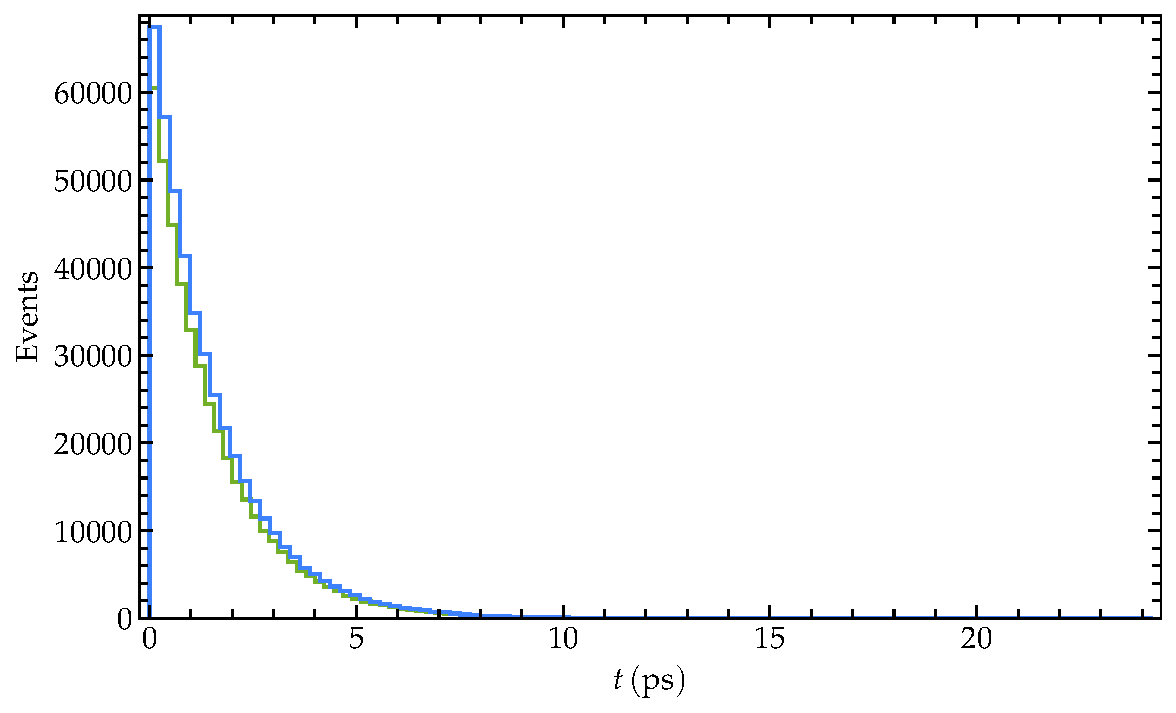
\includegraphics[width=\columnwidth]{plots/time} \\
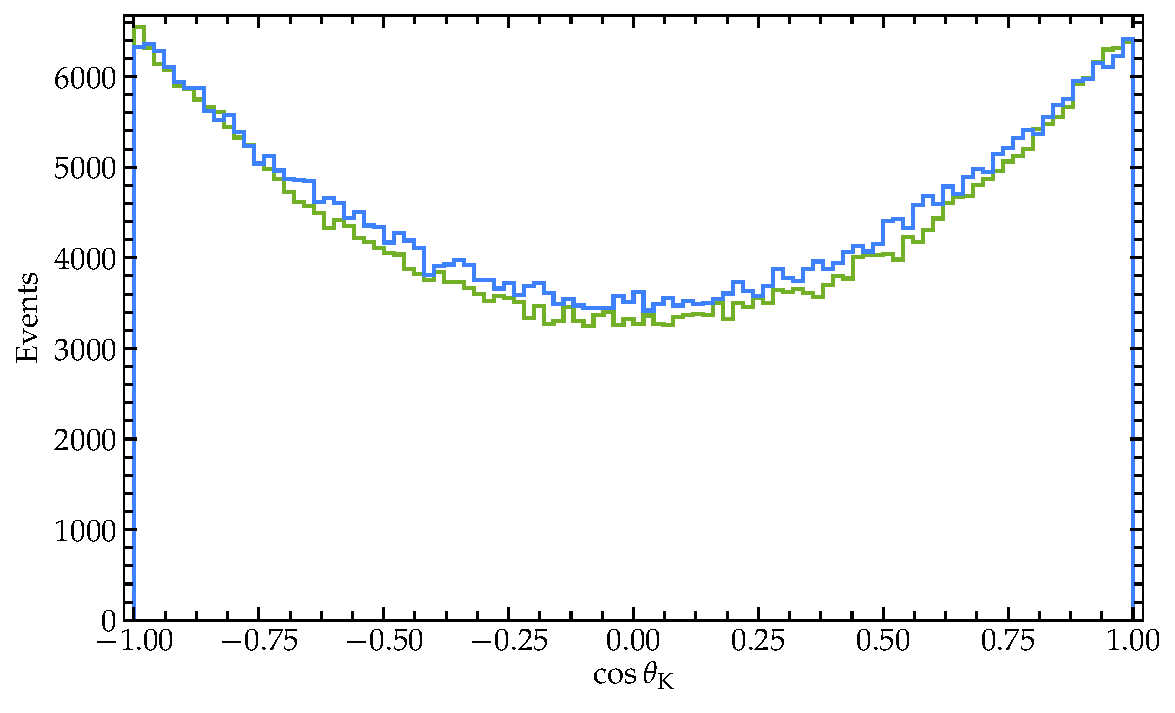
\includegraphics[width=\columnwidth]{plots/hel_costhetaK} \\
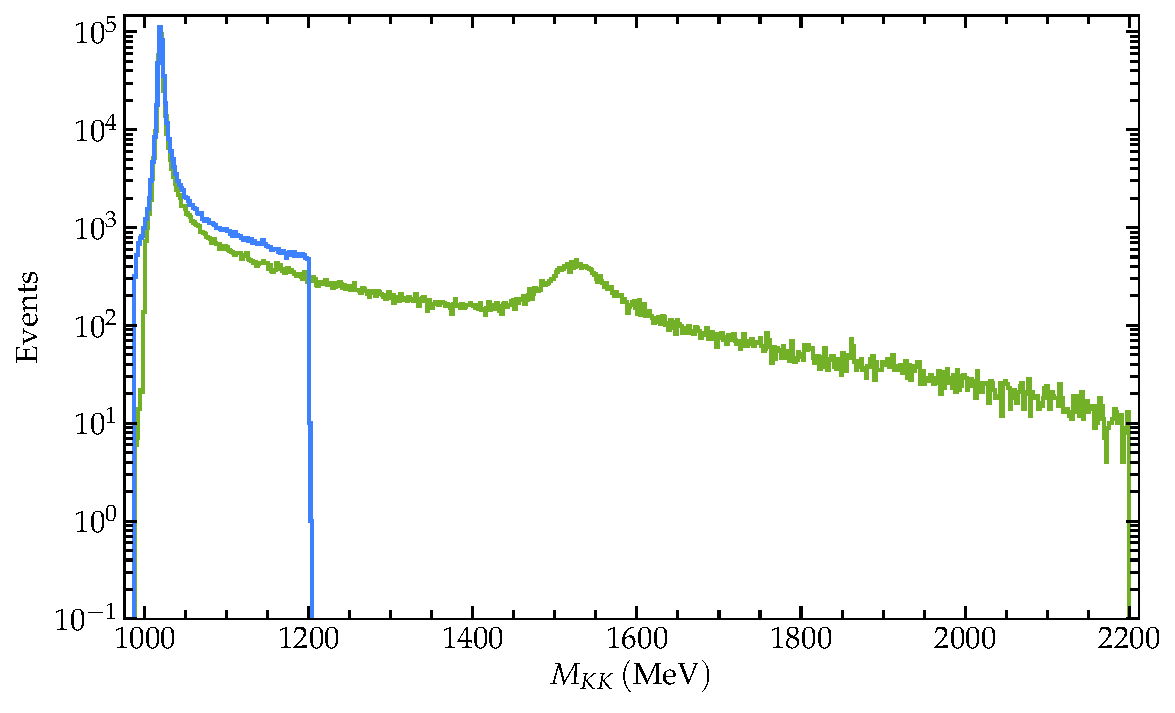
\includegraphics[width=\columnwidth]{plots/mkk} \\
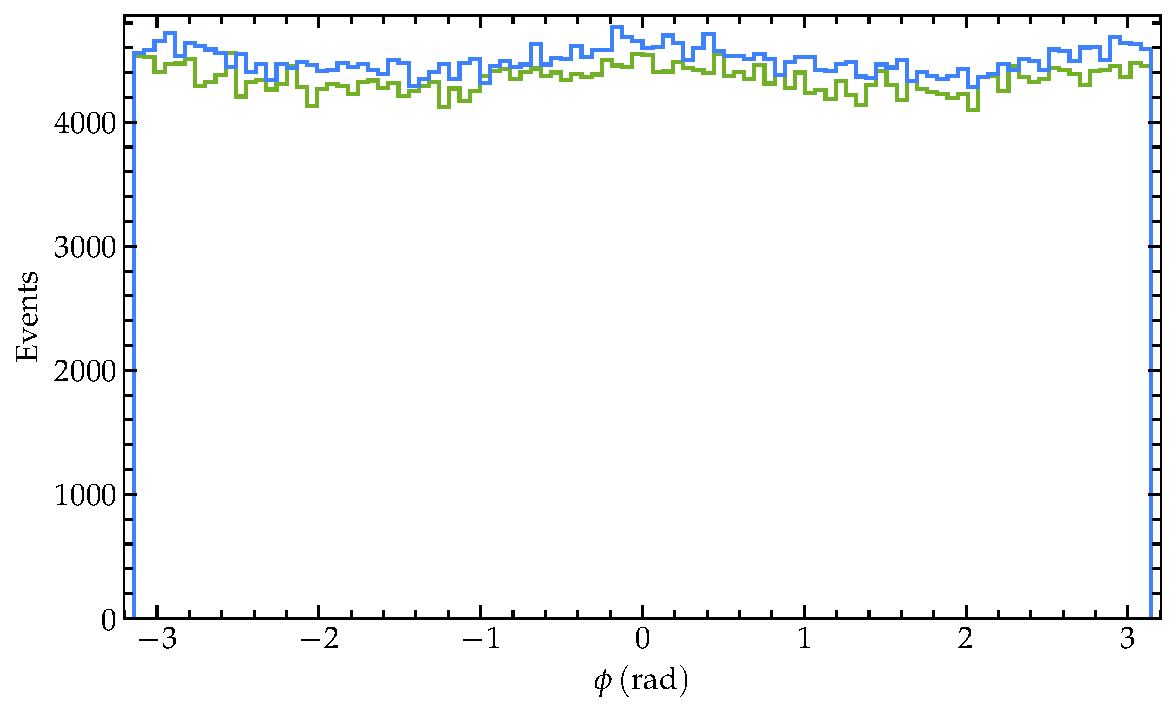
\includegraphics[width=\columnwidth]{plots/hel_phi} \\
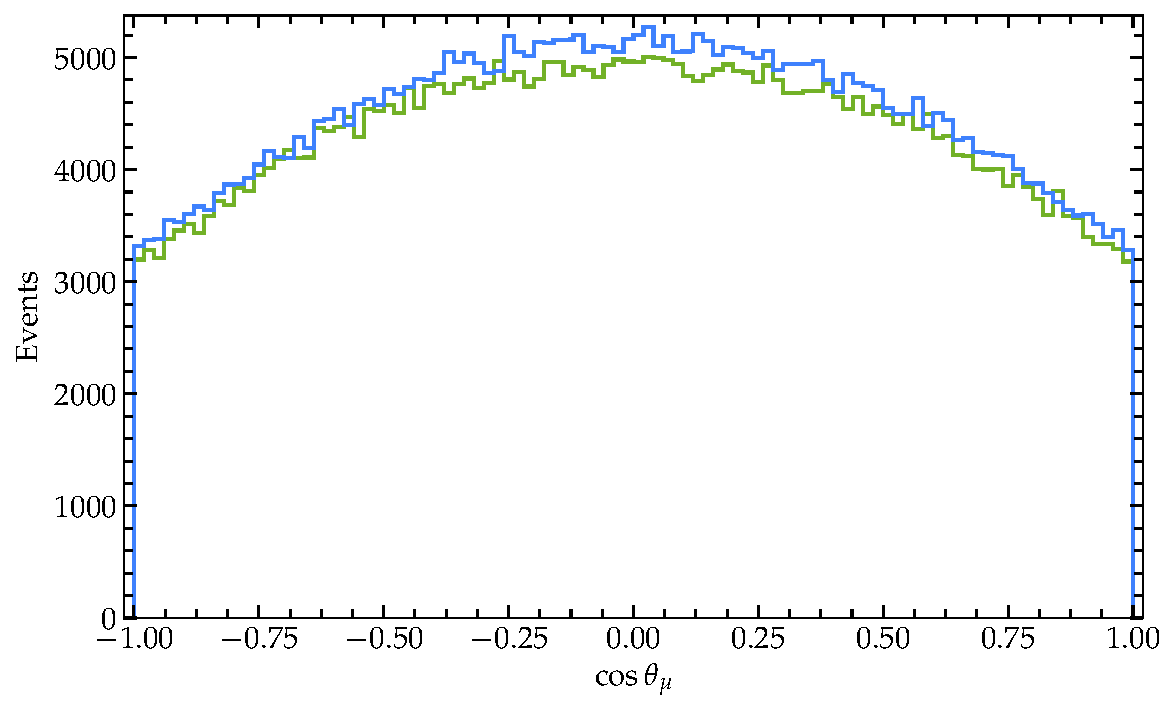
\includegraphics[width=\columnwidth]{plots/hel_costhetamu} \\
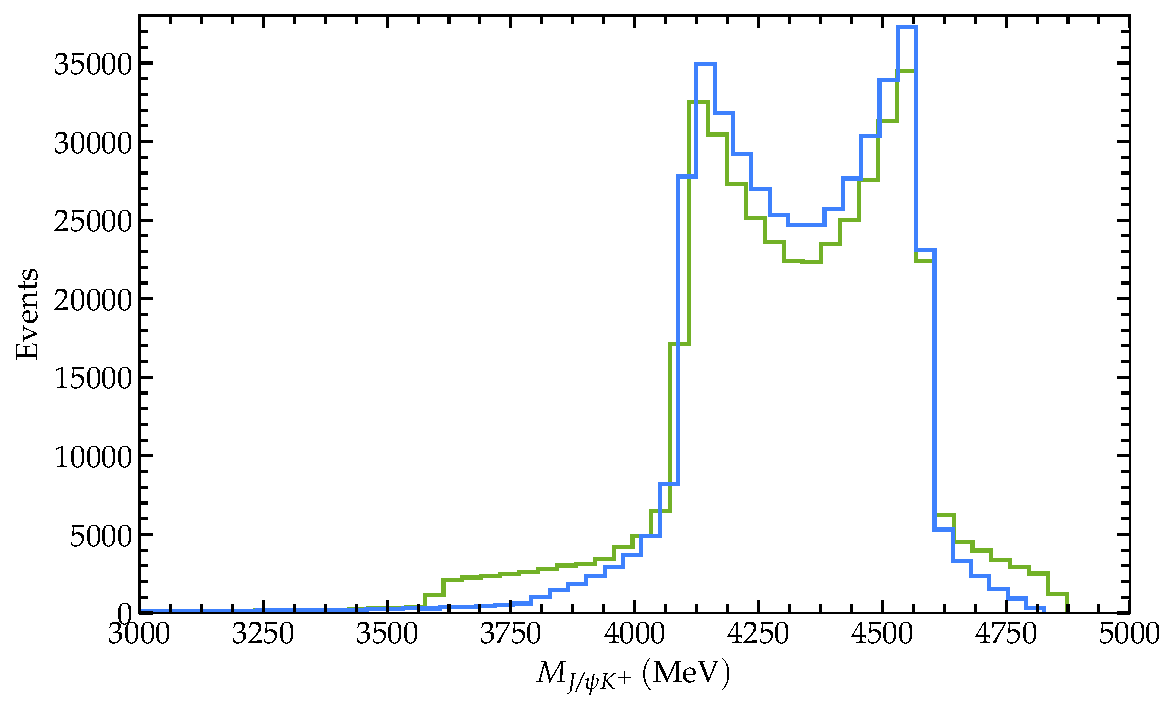
\includegraphics[width=\columnwidth]{plots/mjpsik}
\end{multicols}
\end{flushright}
\caption{Histogramas de algunas de las variables simuladas. Las muestras de $5\times10^5$ eventos  son \emph{sin} onda D (azul), con $7\,\%$ S onda y $93\,\%$ P \emph{wave} en la ventana de masa $m_{\text{KK}} = [0.98,1.20]\,\mathrm{GeV}/c^2$; y \emph{con} onda D (verde), con $15\,\%$ S \emph{wave} y $70\,\%$ P \emph{wave} y $15\,\%$ D \emph{wave} en el rango de masa $m_{\text{KK}} = [1.0,2.2]\,\mathrm{GeV}/c^2$.}   \label{fig_evtgensamples1}
\end{figure}





\begin{figure}[H]
\centering
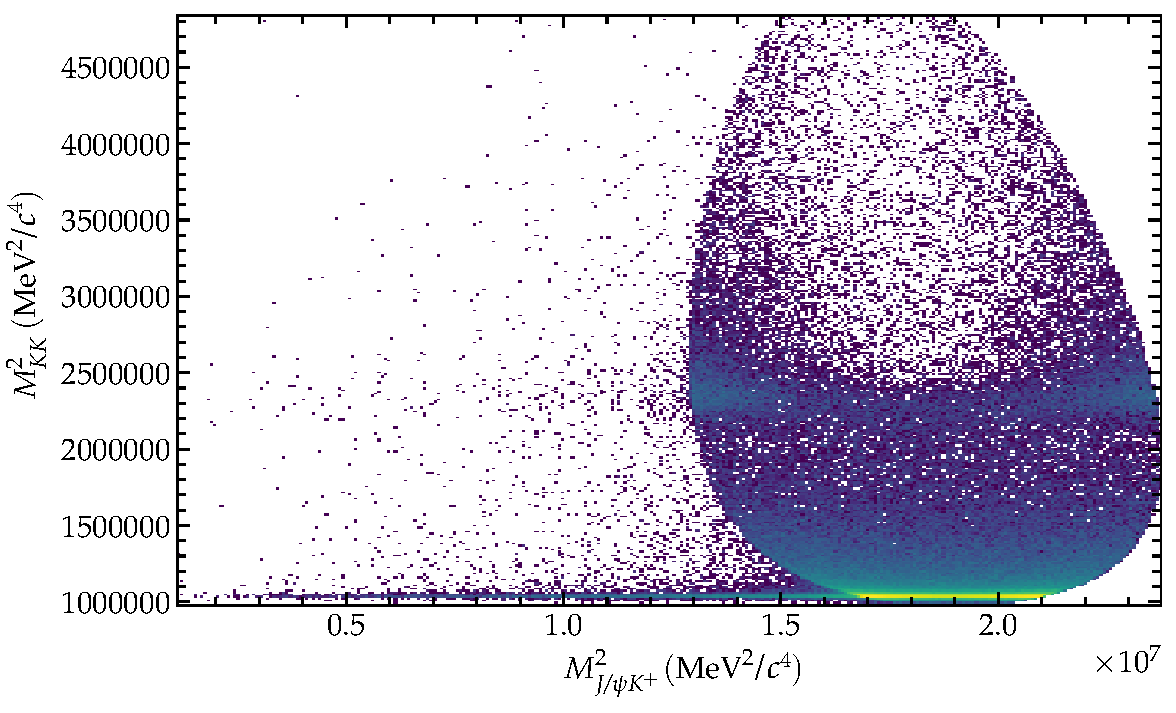
\includegraphics[width=0.9\textwidth]{plots/dalitz1}
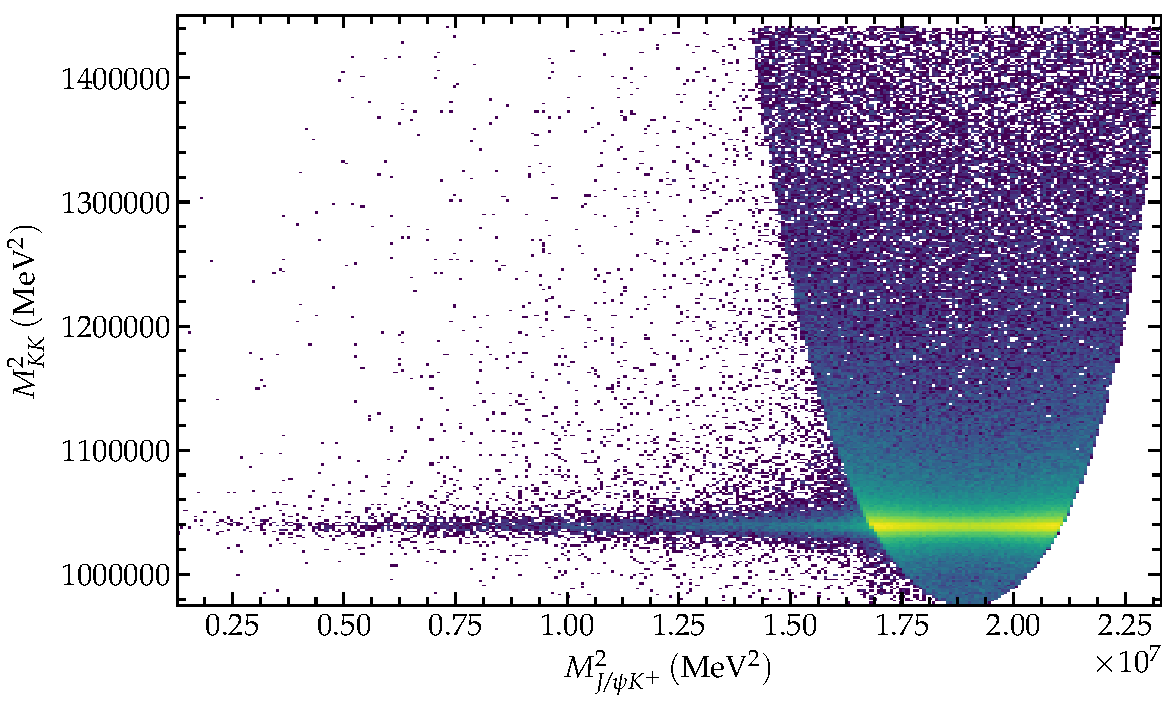
\includegraphics[width=0.9\textwidth]{plots/dalitz2}
\caption{Dalitz \textit{plot} para dos muestra de $5\times 10^5$ eventos, arriba con $15\,\%$ S \emph{wave}, $70\,\%$ P \emph{wave} y $15\,\%$ D \emph{wave} y abajo $11\,\%$ S \emph{wave}, $89\,\%$ P \emph{wave}. Se aprecian claramente las resonancias $\fai$ y $\ftwop$. Alrededor del $\fai$, puede verse también $\fzero$ de una forma más difusa.}   \label{fig_evtgensamples2}
\end{figure}




%%TODO wave -> onda

\section{Comprobación de la simulación}



\subsection{Modelo con ondas S y P}

\begin{table}[H]
\centering
\begin{multicols}{2}
\begin{tabular}{cc}
\toprule
Parámetro & Valor \\ \midrule
$ DG          $&$ 0.0848 \pm 0.0026 $ \\
$ GsmGd       $&$0.00093 \pm 0.00082$ \\
$ DM          $&$ 17.6974 \pm 0.0023$ \\
$ phisPlon    $&$ -0.0313 \pm 0.0022$ \\
$ lamPlon     $&$ 0.9994 \pm 0.0015 $ \\
$ fPlon       $&$0.51348 \pm 0.00095$ \\
$ fPper       $&$ 0.2531 \pm 0.0012 $ \\
$ dPpar       $&$ 3.2576 \pm 0.0084 $ \\
$ dPper       $&$ 3.0794 \pm 0.0069 $ \\
\bottomrule
\end{tabular}
\begin{tabular}{cc}
\toprule
Parámetro & Valor \\ \midrule
$ FS_mKK1     $&$  0.482 \pm 0.011  $ \\
$ FS_mKK2     $&$ 0.0515 \pm 0.0015 $ \\
$ FS_mKK3     $&$ 0.0061 \pm 0.00026$ \\
$ FS_mKK4     $&$0.00897 \pm 0.00038$ \\
$ FS_mKK5     $&$ 0.0429 \pm 0.0013 $ \\
$ FS_mKK6     $&$  0.1504 \pm 0.003 $ \\
$ dSlon_mKK1  $&$  1.825 \pm 0.016  $ \\
$ dSlon_mKK2  $&$  1.642 \pm 0.017  $ \\
$ dSlon_mKK3  $&$   0.88 \pm 0.023  $ \\
$ dSlon_mKK4  $&$  -0.356 \pm 0.02  $ \\
$ dSlon_mKK5  $&$  -0.807 \pm 0.015 $ \\
$ dSlon_mKK6  $&$  -0.925 \pm 0.011 $ \\
\bottomrule
\end{tabular}
\end{multicols}
  \caption{Valores obtenidos del ajuste a una muestra de un millón de eventos  de MC.}
\end{table}

%+---------------+--------------------+
%| Fit Parameter | Value ± ParabError |
%+---------------+--------------------+
%| DG            |  0.0848 ± 0.0026   |
%| GsmGd         | 0.00093 ± 0.00082  |
%| DM            |  17.6974 ± 0.0023  |
%| fPlon         | 0.51348 ± 0.00095  |
%| fPper         |  0.2531 ± 0.0012   |
%| FS_mKK1       |   0.482 ± 0.011    |
%| FS_mKK2       |  0.0515 ± 0.0015   |
%| FS_mKK3       |  0.0061 ± 0.00026  |
%| FS_mKK4       | 0.00897 ± 0.00038  |
%| FS_mKK5       |  0.0429 ± 0.0013   |
%| FS_mKK6       |   0.1504 ± 0.003   |
%| dPpar         |  3.2576 ± 0.0084   |
%| dPper         |  3.0794 ± 0.0069   |
%| dSlon_mKK1    |   1.825 ± 0.016    |
%| dSlon_mKK2    |   1.642 ± 0.017    |
%| dSlon_mKK3    |    0.88 ± 0.023    |
%| dSlon_mKK4    |   -0.356 ± 0.02    |
%| dSlon_mKK5    |   -0.807 ± 0.015   |
%| dSlon_mKK6    |   -0.925 ± 0.011   |
%| phisPlon      |  -0.0313 ± 0.0022  |
%| lamPlon       |  0.9994 ± 0.0015   |
%+---------------+--------------------+



\subsection{Modelo con ondas S, P y D}

Se escribió
%, en parte para comprobar los resultados del MC de la \S \ref{sec:Bs2JpsiKKmodel}, 
un programa capaz de ajustar muestras de datos con onda D. Esto incluye, evidentemente, ajustar un conjunto de parámetros más grande, y que en su máxima amplitud resulta en 76.

El algoritmo, diseñado para correr en GPU, funciona correctamente y valida los parámetros impuestos al generador de las muestras de MC. Corriendo sobre una \textsc{nVidia GeForce GTX 1080 Ti}, se puede ajustar una muestra de $0.5$ millones de eventos, en aproximadamente $6$ minutos, incluyendo la carga de los datos, el tiempo de minimización, y la salida de los resultados (Tabla \ref{tab:fitDwaveparams}) y gráficas (Figuras \ref{fig:20190221c_mKK1} a \ref{fig:20190221c_mKK6}).











\begin{table}[H]
\centering
\begin{multicols}{2}
\begin{tabular}{cc}
\toprule
Parámetro & Valor \\ \midrule
$DG        $&$ 0.0796 \pm 0.0035  $\\
$GsmGd     $&$ 0.0005 \pm 0.0011  $\\
$DM        $&$ 17.7054 \pm 0.0032 $\\
$phisPlon  $&$ -0.0323 \pm 0.0032 $\\
$lamPlon   $&$  0.9996 \pm 0.002  $\\
$fPlon     $&$ 0.5116 \pm 0.0014  $\\
$fPper     $&$ 0.2558 \pm 0.0018  $\\
$fDlon     $&$   0.5 \pm 0.0003   $\\
$fDper     $&$  0.2 \pm 0.00059   $\\
$FS_mKK1   $&$0.01624 \pm 0.00072 $\\
$FS_mKK2   $&$ 0.4253 \pm 0.0091  $\\
$FS_mKK3   $&$   0.194 \pm 0.01   $\\
$FS_mKK4   $&$  0.261 \pm 0.016   $\\
$FS_mKK5   $&$  0.254 \pm 0.023   $\\
$FS_mKK6   $&$  0.316 \pm 0.031   $\\
$FD_mKK1   $&$0.000446 \pm 8.7e-05$\\
$FD_mKK2   $&$  0.0414 \pm 0.003  $\\
$FD_mKK3   $&$  0.631 \pm 0.011   $\\
$FD_mKK4   $&$  0.314 \pm 0.013   $\\
$FD_mKK5   $&$  0.184 \pm 0.014   $\\
$FD_mKK6   $&$   0.15 \pm 0.017   $\\
$dPpar     $&$   3.1 \pm 0.012    $\\
$dPper     $&$  2.9271 \pm 0.009  $\\
\bottomrule
\end{tabular}
\begin{tabular}{cc}
\toprule
Parámetro & Valor \\ \midrule
$dSlon_mKK1$&$ 1e-05 \pm 0.00048  $\\
$dSlon_mKK2$&$ 1e-05 \pm 0.00028  $\\
$dSlon_mKK3$&$   0.0 \pm 0.0026   $\\
$dSlon_mKK4$&$  -0.123 \pm 0.028  $\\
$dSlon_mKK5$&$  -0.135 \pm 0.038  $\\
$dSlon_mKK6$&$  -0.107 \pm 0.052  $\\
$dDlon_mKK1$&$   -2.97 \pm 0.1    $\\
$dDlon_mKK2$&$  -2.09 \pm 0.039   $\\
$dDlon_mKK3$&$  -1.54 \pm 0.014   $\\
$dDlon_mKK4$&$   -0.2 \pm 0.038   $\\
$dDlon_mKK5$&$  -0.03 \pm 0.058   $\\
$dDlon_mKK6$&$  0.064 \pm 0.097   $\\
$dDper_mKK1$&$  -6.283 \pm 0.014  $\\
$dDper_mKK2$&$ -6.2832 \pm 0.003  $\\
$dDper_mKK3$&$  -0.766 \pm 0.035  $\\
$dDper_mKK4$&$  0.503 \pm 0.063   $\\
$dDper_mKK5$&$   1.07 \pm 0.12    $\\
$dDper_mKK6$&$   0.58 \pm 0.19    $\\
$dDpar_mKK1$&$   0.83 \pm 0.14    $\\
$dDpar_mKK2$&$  1.707 \pm 0.061   $\\
$dDpar_mKK3$&$   2.49 \pm 0.034   $\\
$dDpar_mKK4$&$  -2.435 \pm 0.049  $\\
$dDpar_mKK5$&$  -2.372 \pm 0.09   $\\
$dDpar_mKK6$&$   -2.29 \pm 0.13   $\\
\bottomrule
\end{tabular}
\end{multicols}
  \caption{Valores obtenidos del ajuste a una muestra de un millón de eventos  de MC.} \label{tab:fitDwaveparams}
\end{table}

En las Figuras \ref{fig:20190221c_mKK1}--\ref{fig:20190221c_mKK6} pueden verse las gráficas de los ajustes para cada bin de masa de los definidos.

\newpage

\begin{figure}[H]
\centering
\begin{multicols}{2}
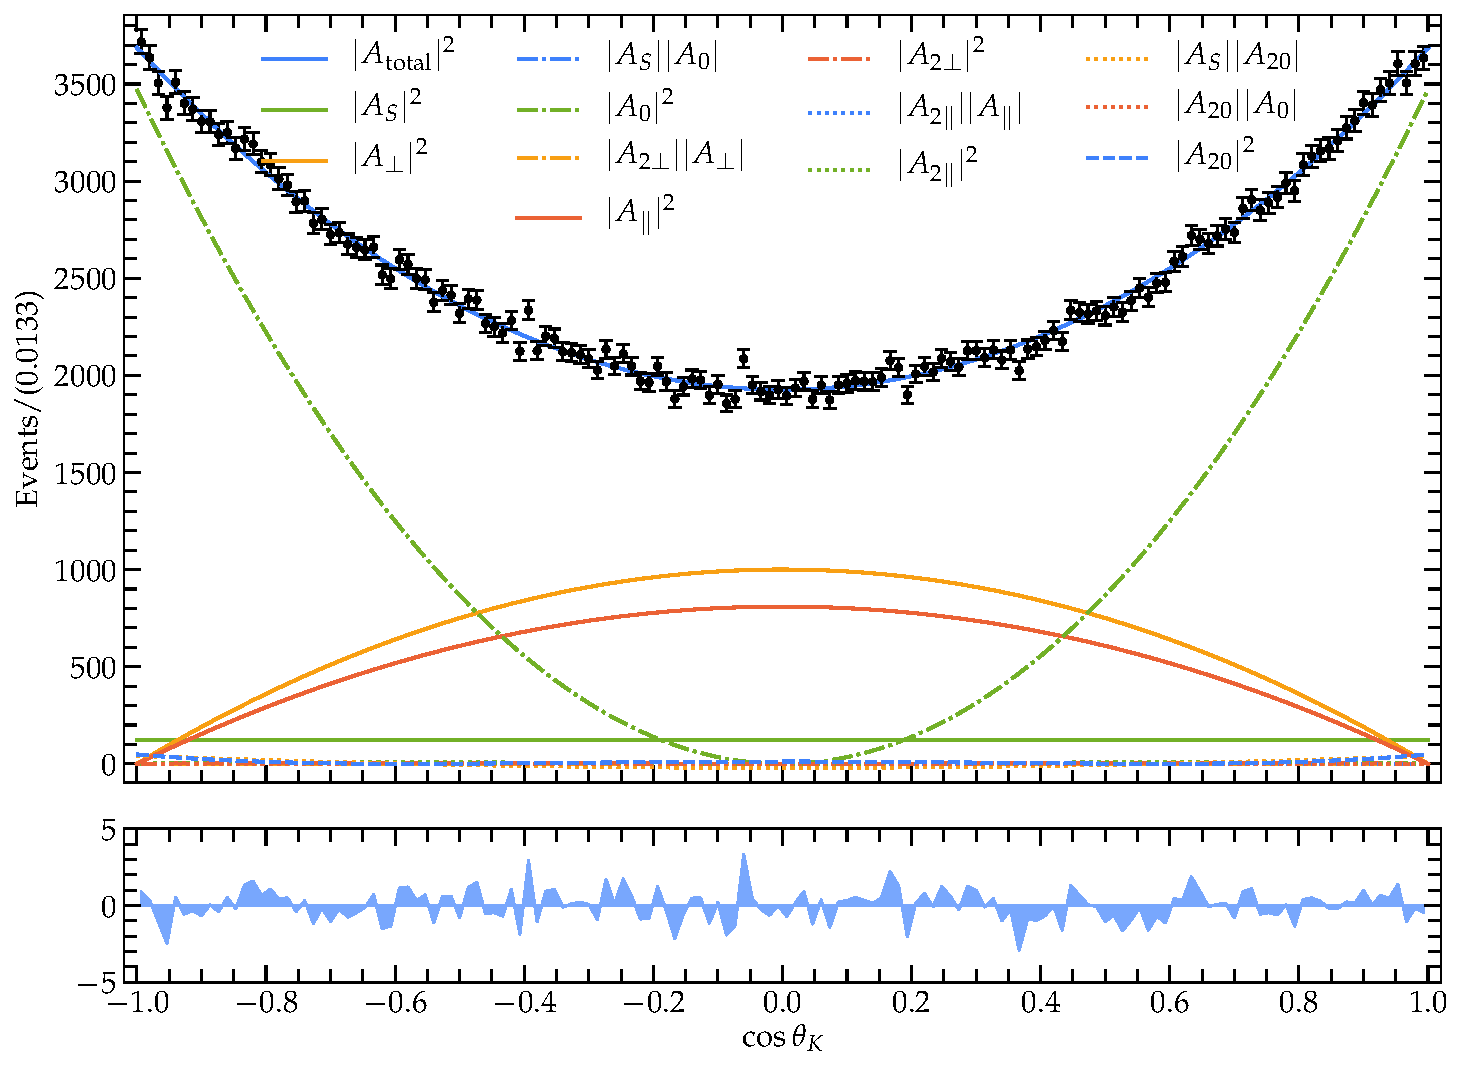
\includegraphics[width=\columnwidth]{plots/20190221c/20190221c_mKK1_CosK}
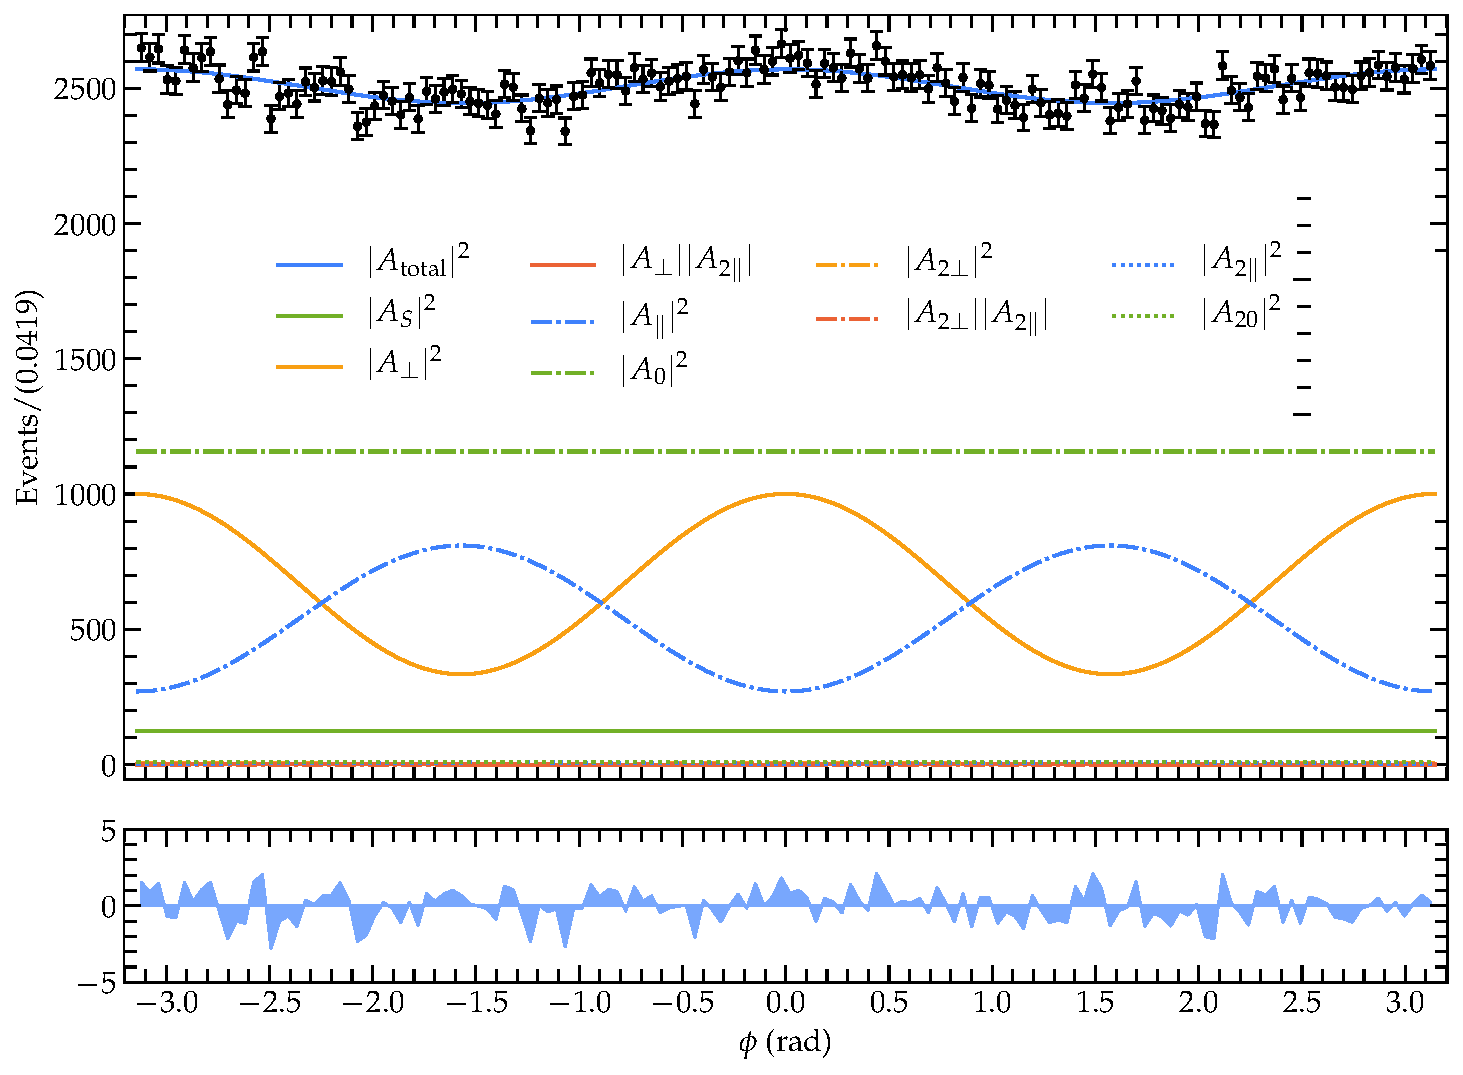
\includegraphics[width=\columnwidth]{plots/20190221c/20190221c_mKK1_Phi}
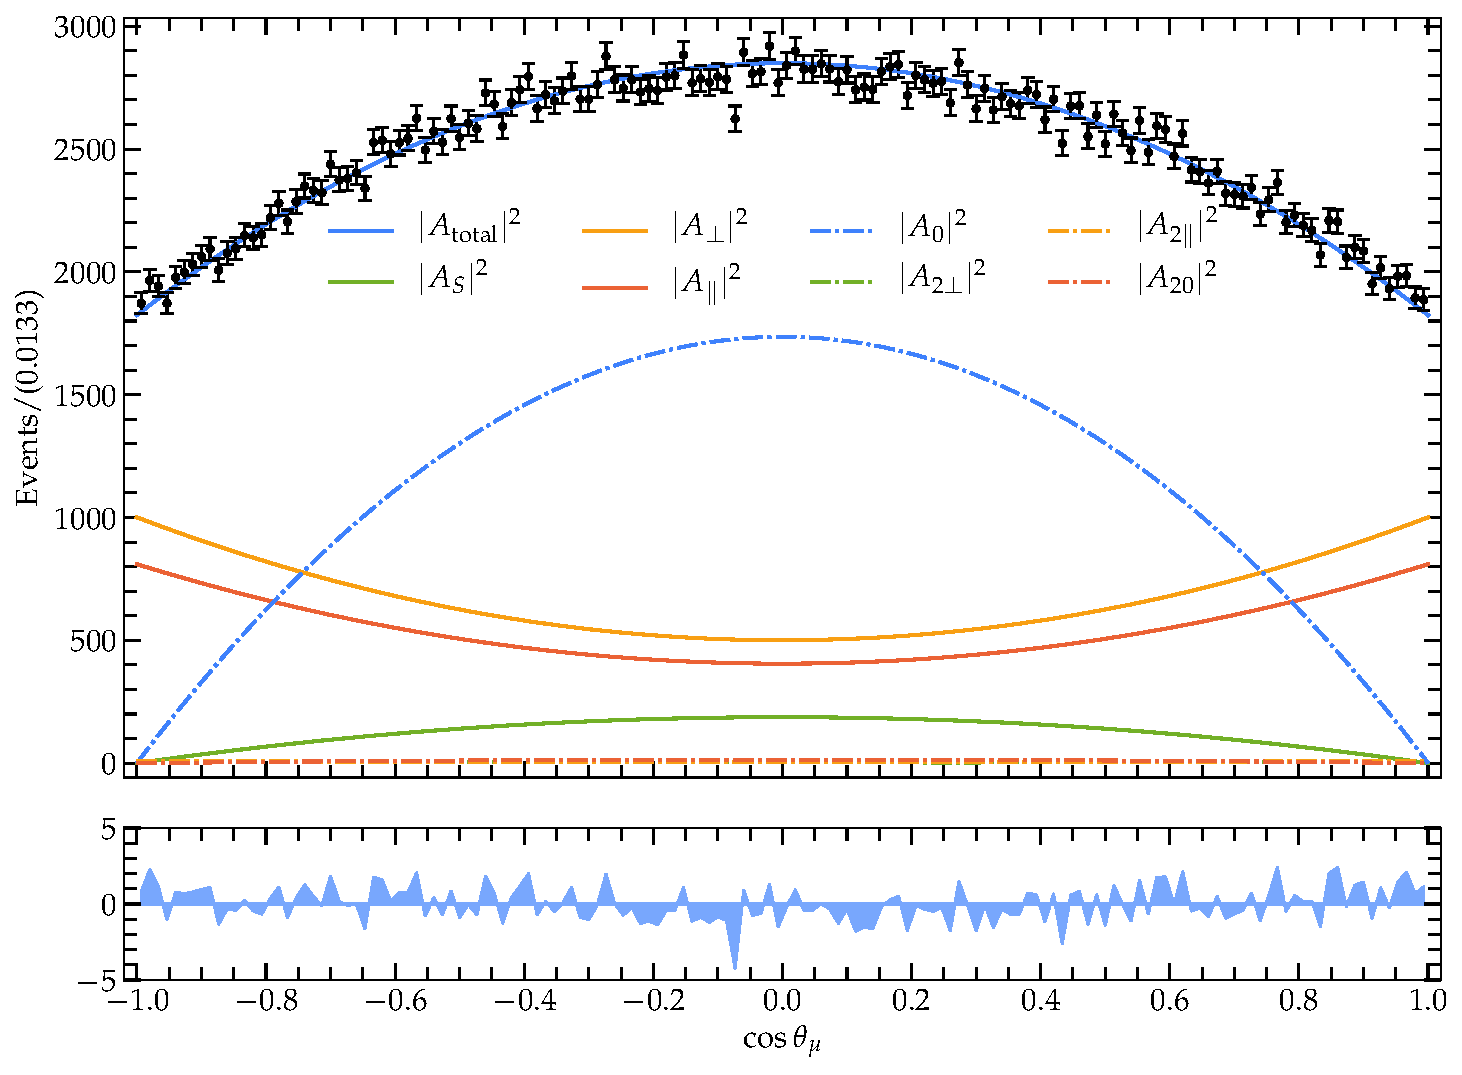
\includegraphics[width=\columnwidth]{plots/20190221c/20190221c_mKK1_CosMu}
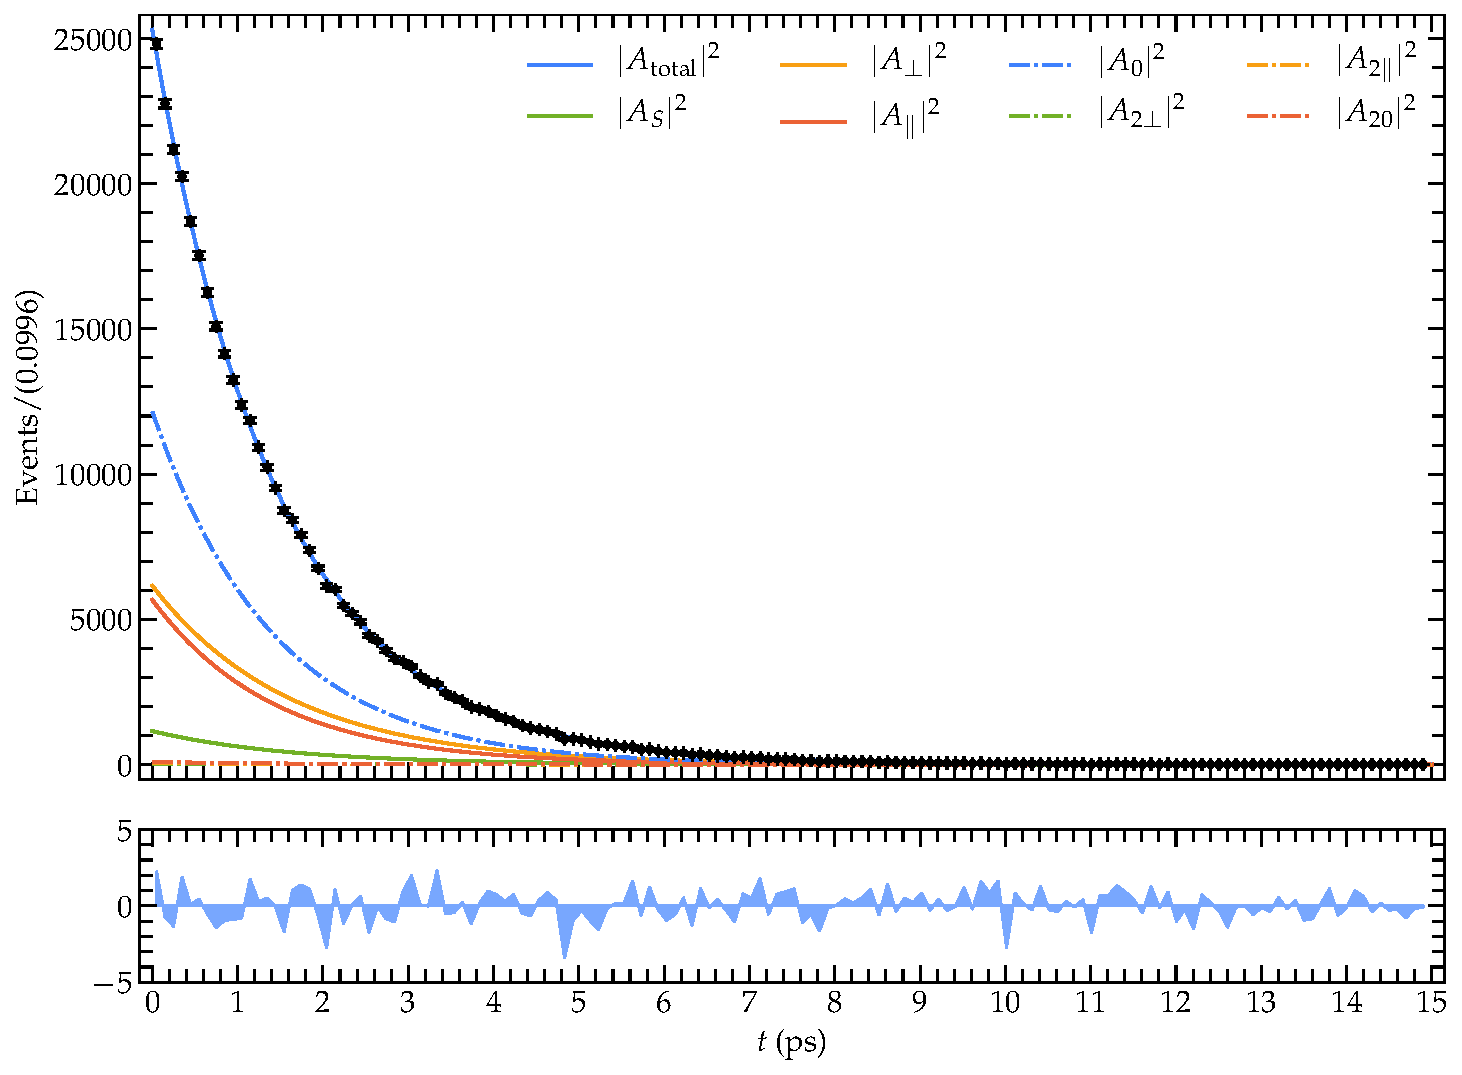
\includegraphics[width=\columnwidth]{plots/20190221c/20190221c_mKK1_Time}
\end{multicols}
\vspace*{-0.5cm}
\caption{Gráficos del ajuste con onda D para el bin $m_{\text{KK}1} = [1.0,1.2)$ GeV.}  \label{fig:20190221c_mKK1}
\end{figure}

\begin{figure}[H]
\centering
\begin{multicols}{2}
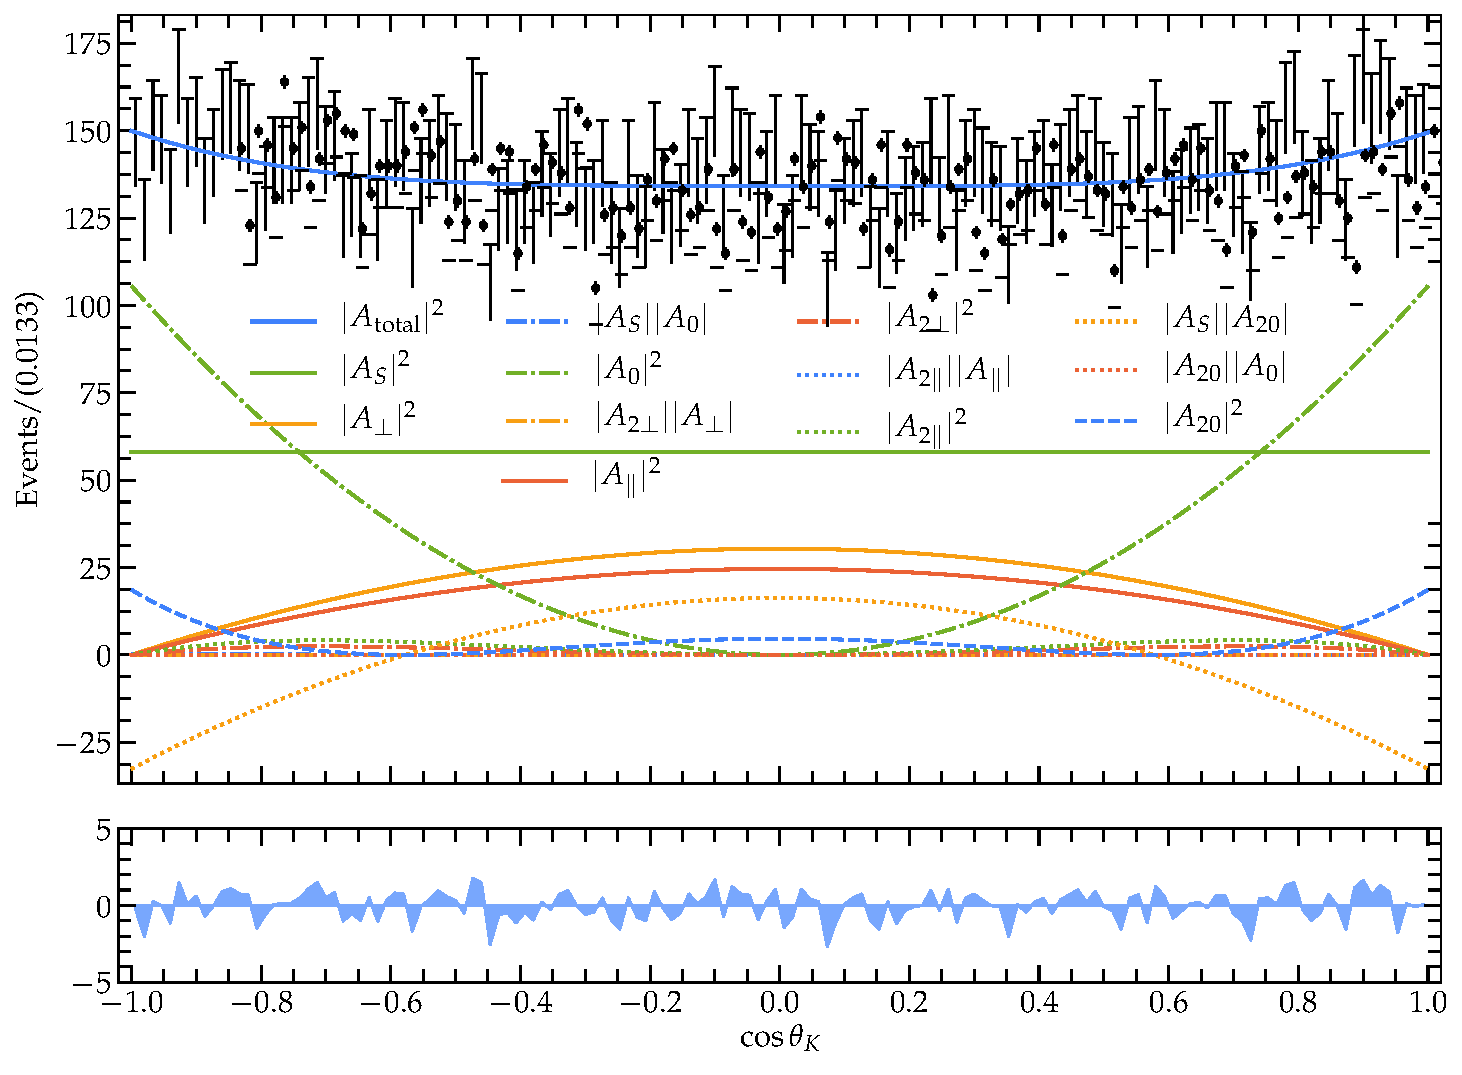
\includegraphics[width=\columnwidth]{plots/20190221c/20190221c_mKK2_CosK}
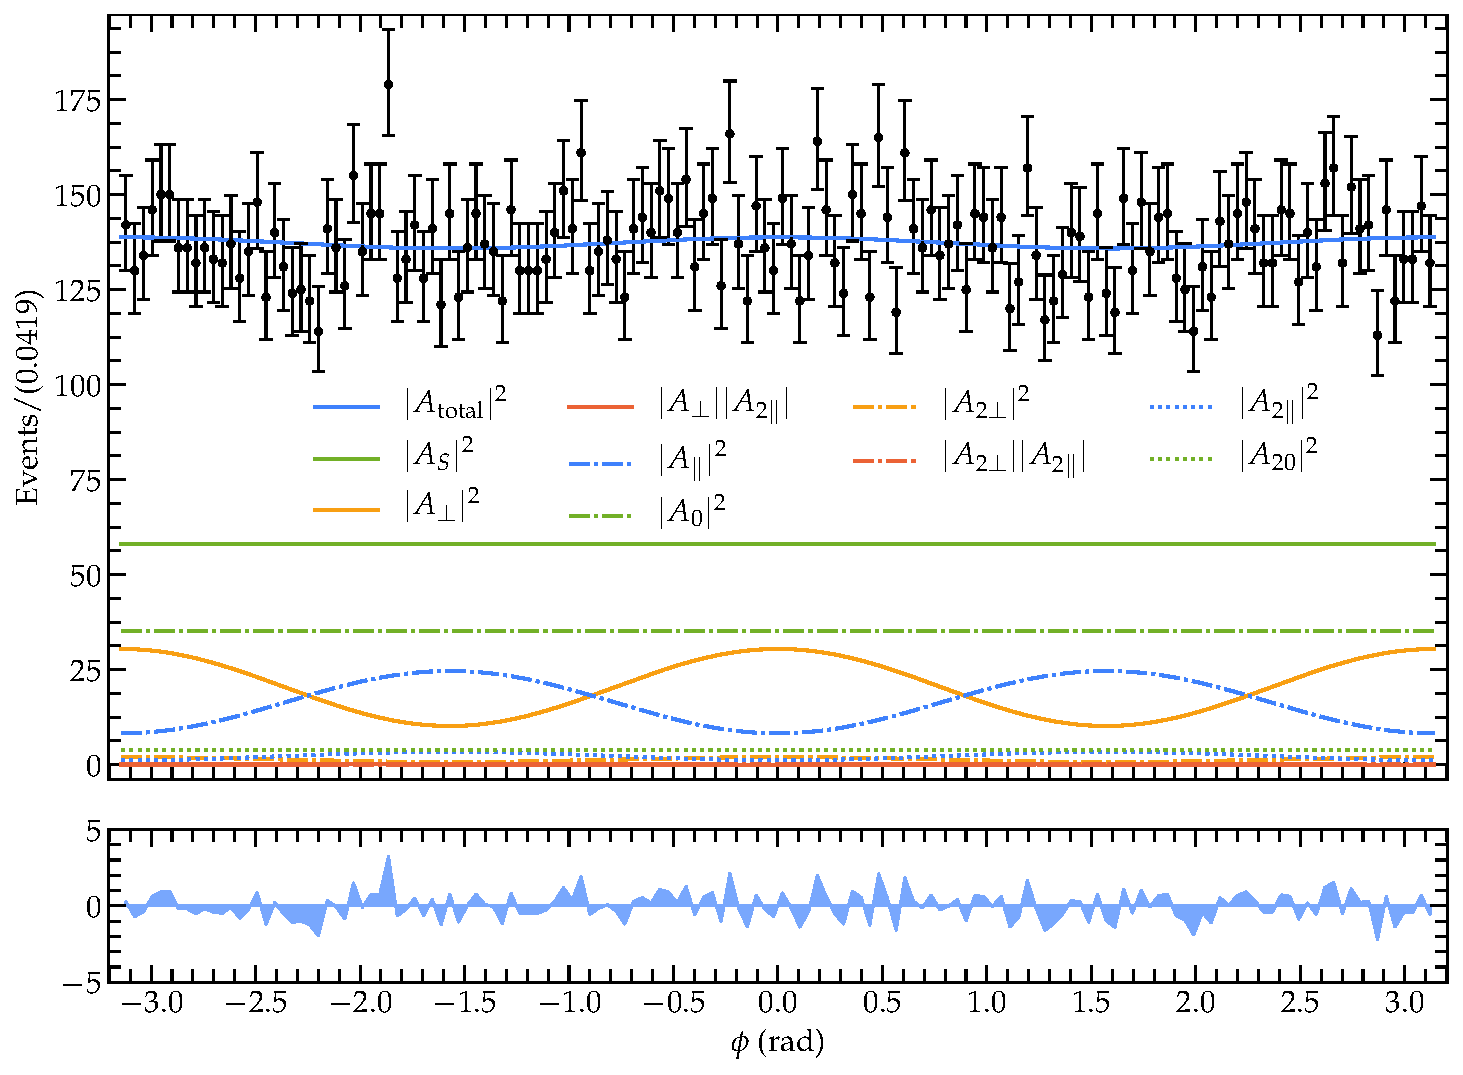
\includegraphics[width=\columnwidth]{plots/20190221c/20190221c_mKK2_Phi}
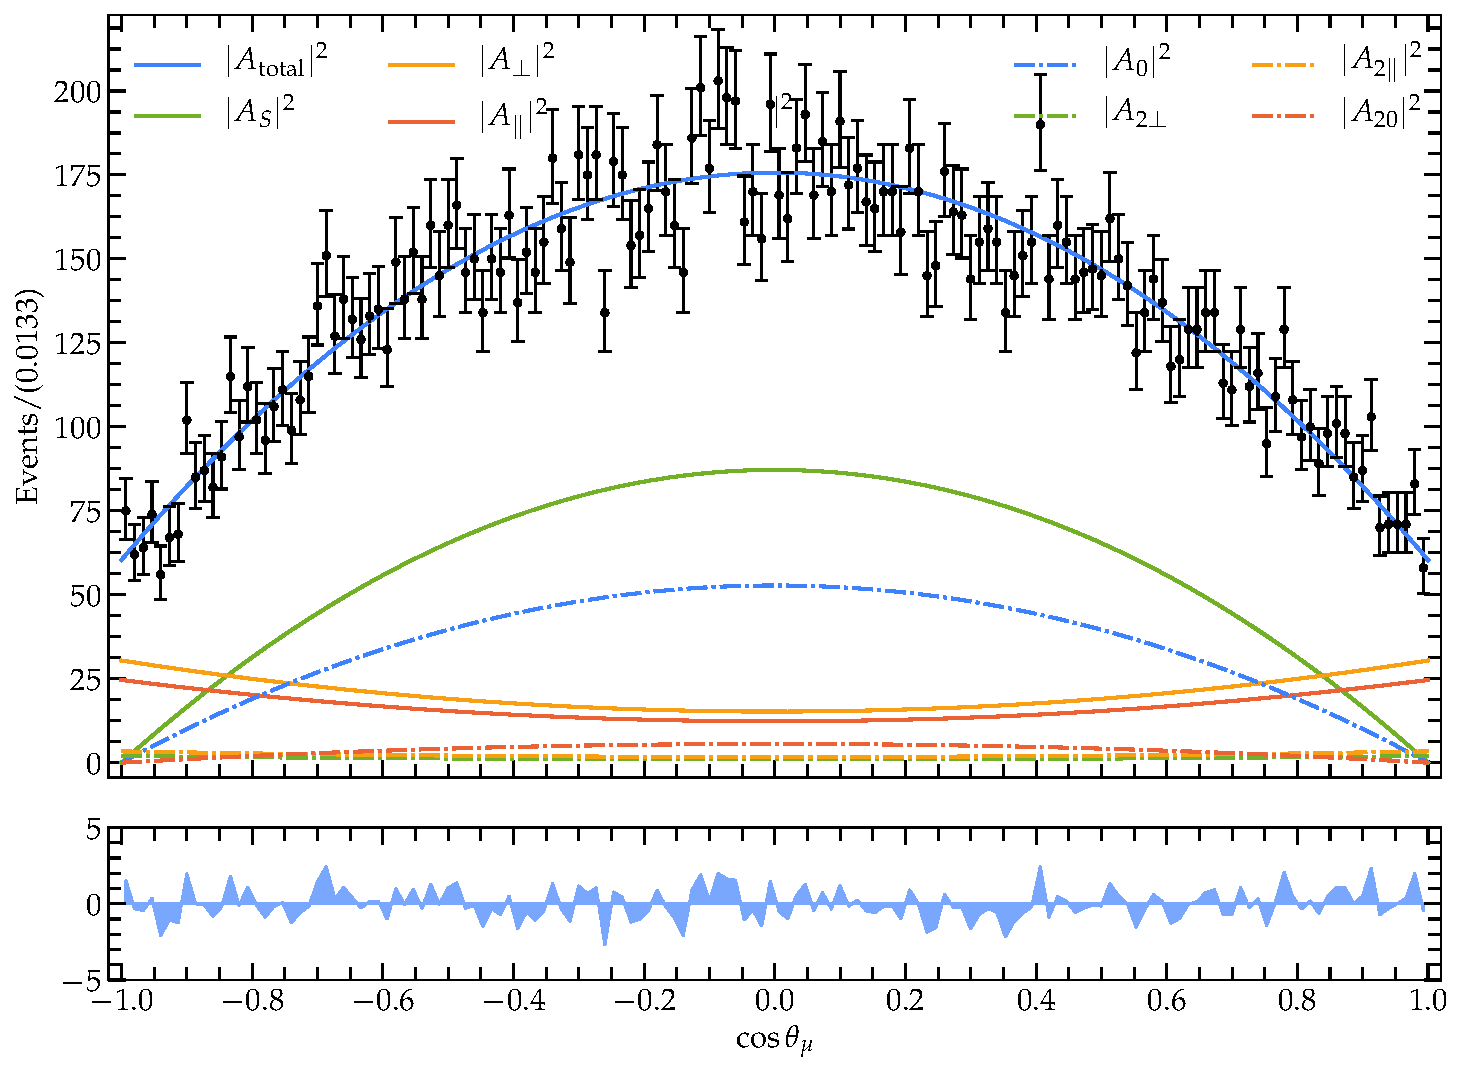
\includegraphics[width=\columnwidth]{plots/20190221c/20190221c_mKK2_CosMu}
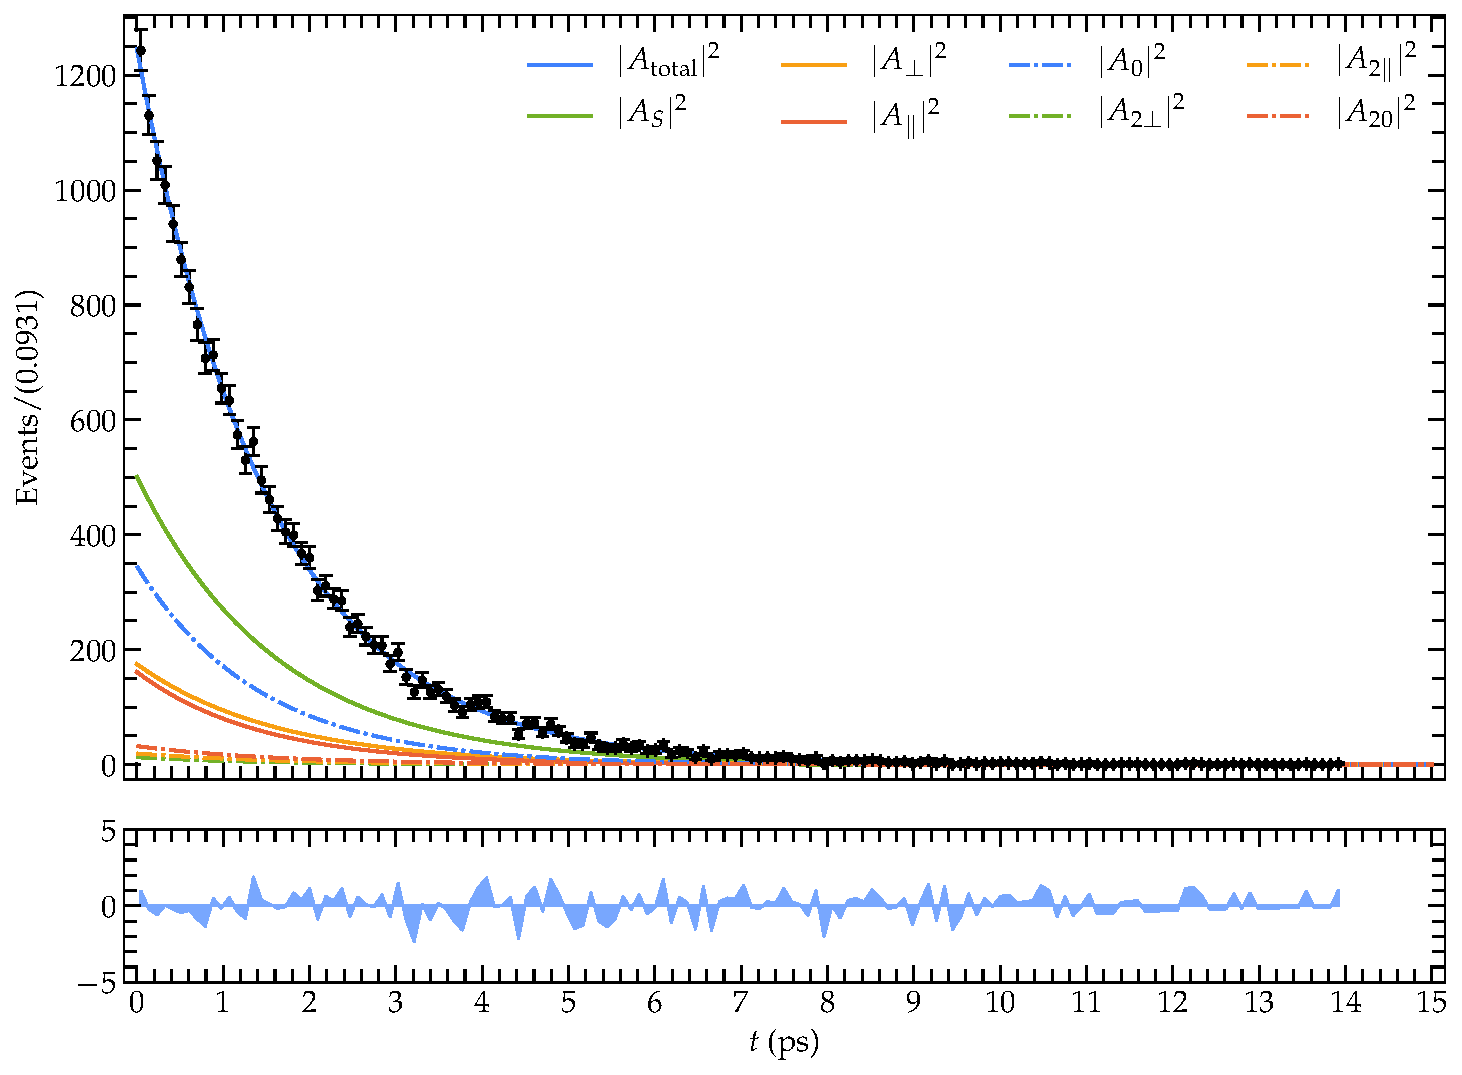
\includegraphics[width=\columnwidth]{plots/20190221c/20190221c_mKK2_Time}
\end{multicols}
\vspace*{-0.5cm}
\caption{Gráficos del ajuste con onda D para el bin $m_{\text{KK}2} = [1.2,1.4)$ GeV.}  
\end{figure}

\begin{figure}[H]
\centering
\begin{multicols}{2}
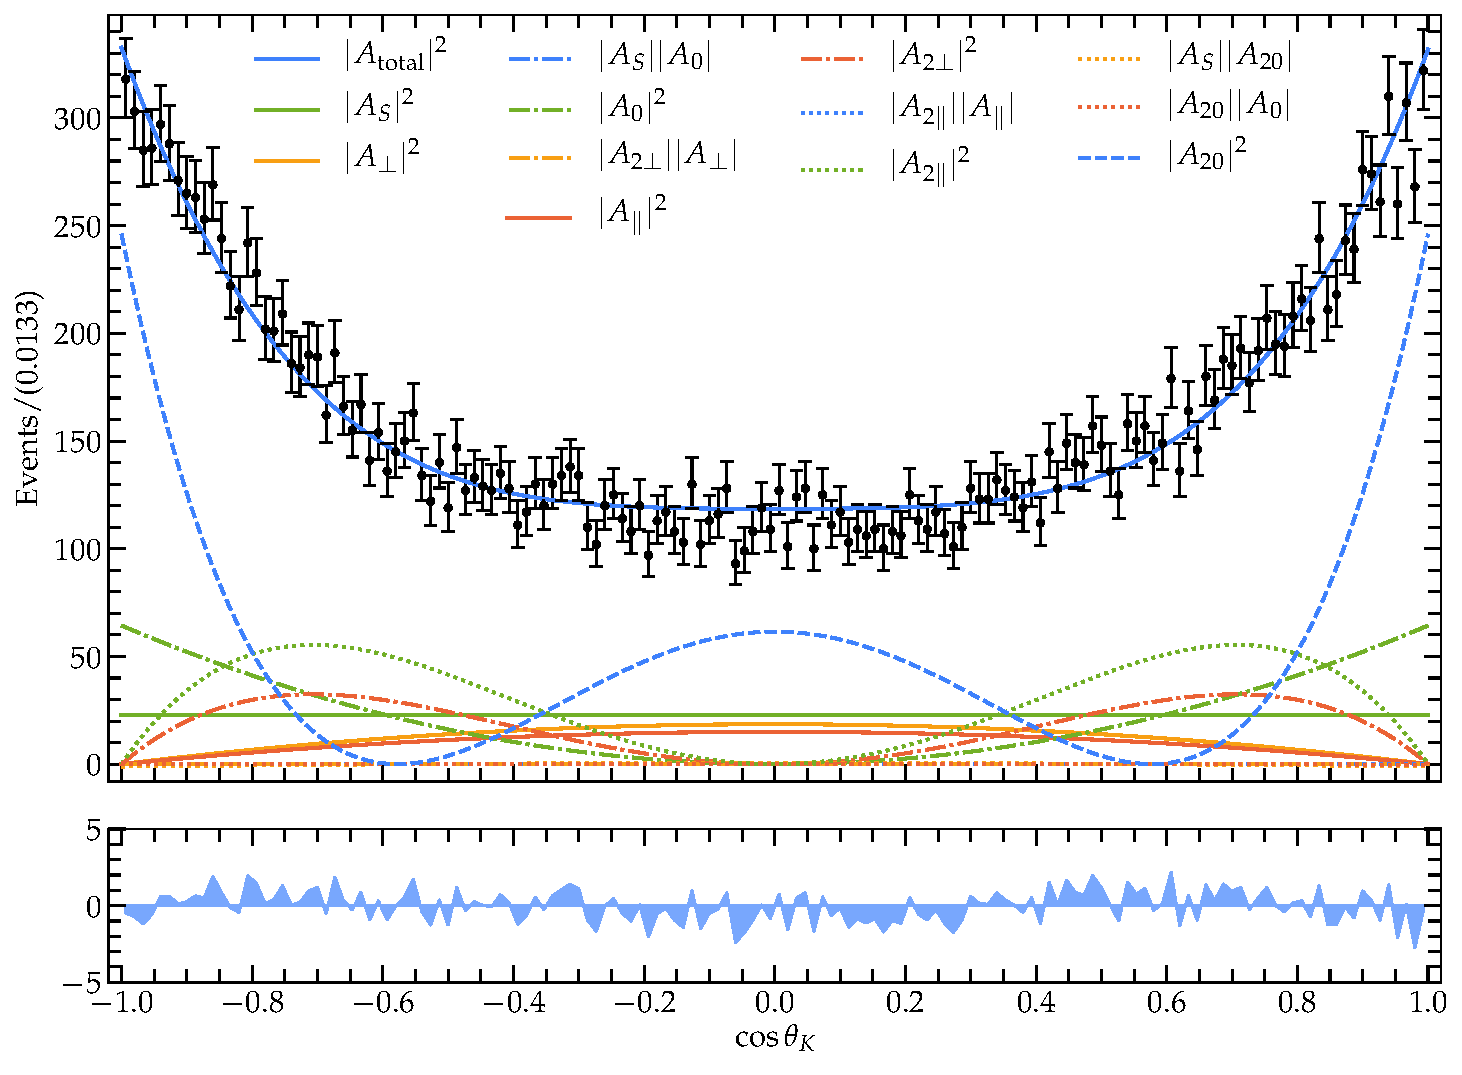
\includegraphics[width=\columnwidth]{plots/20190221c/20190221c_mKK3_CosK}
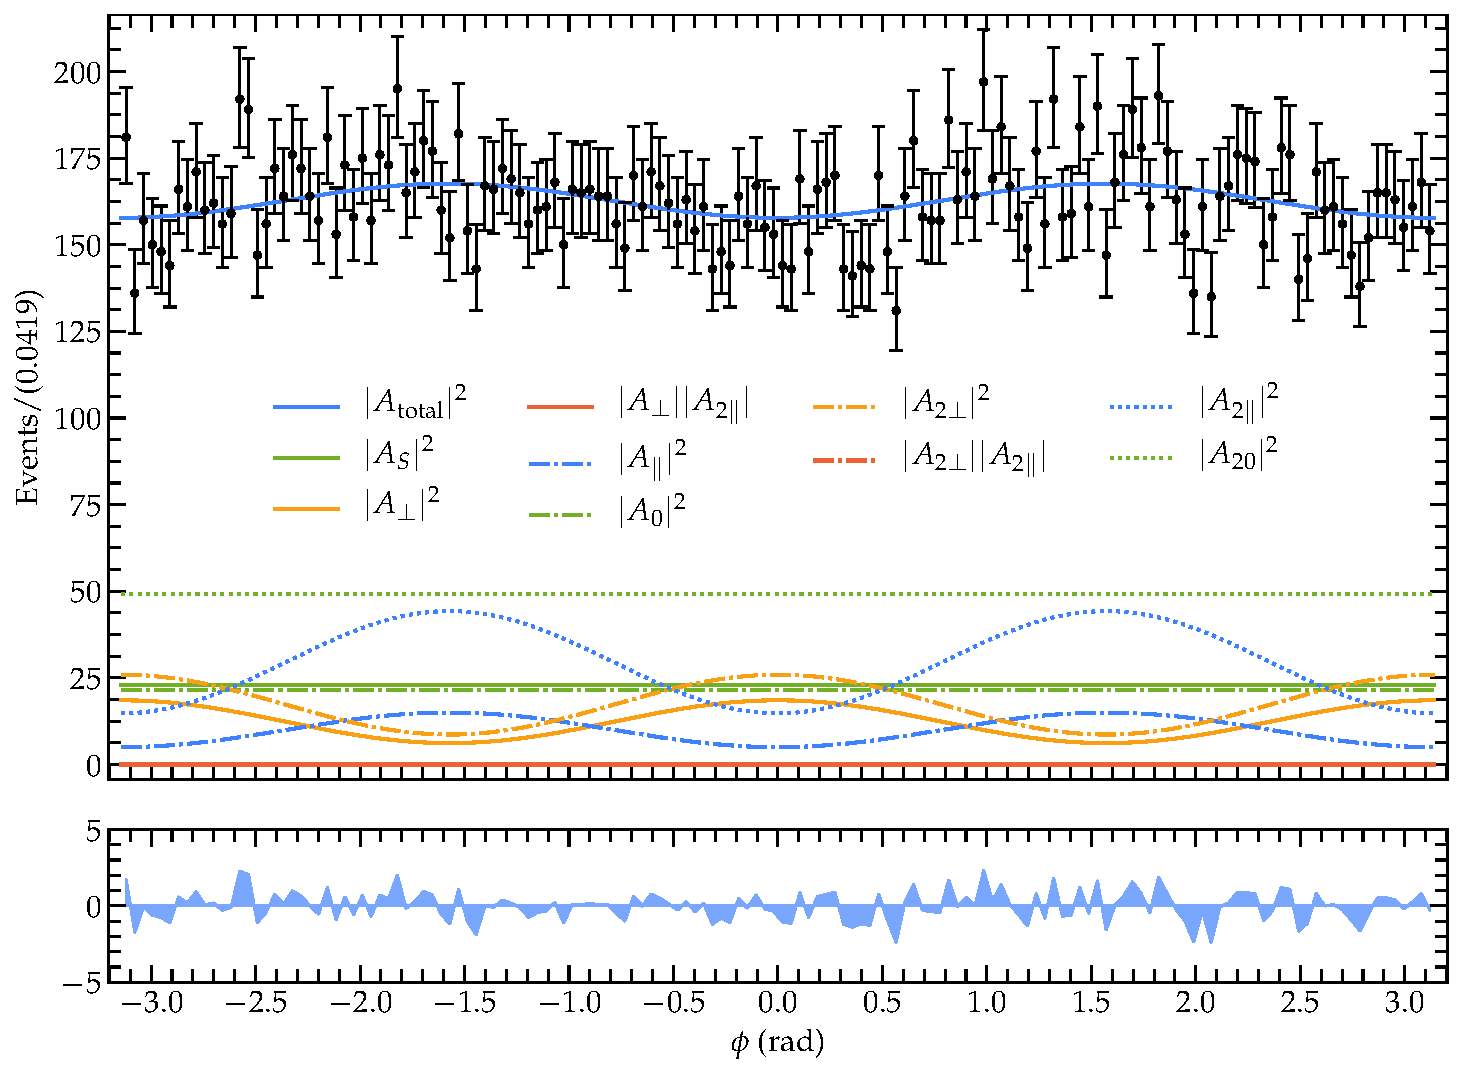
\includegraphics[width=\columnwidth]{plots/20190221c/20190221c_mKK3_Phi}
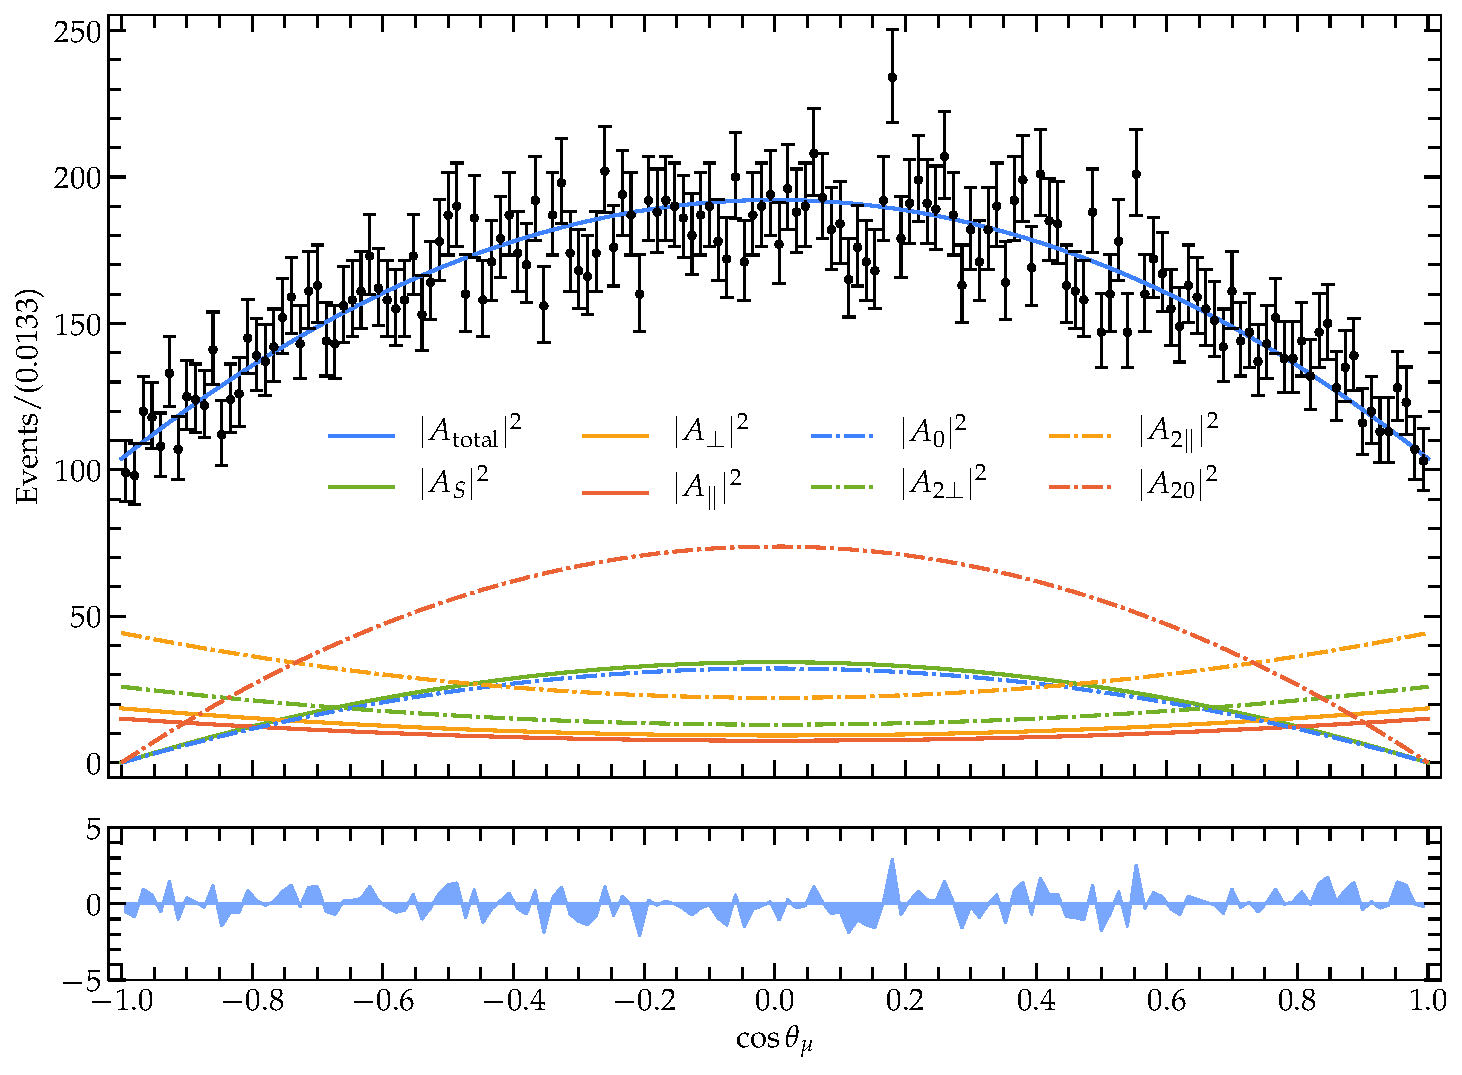
\includegraphics[width=\columnwidth]{plots/20190221c/20190221c_mKK3_CosMu}
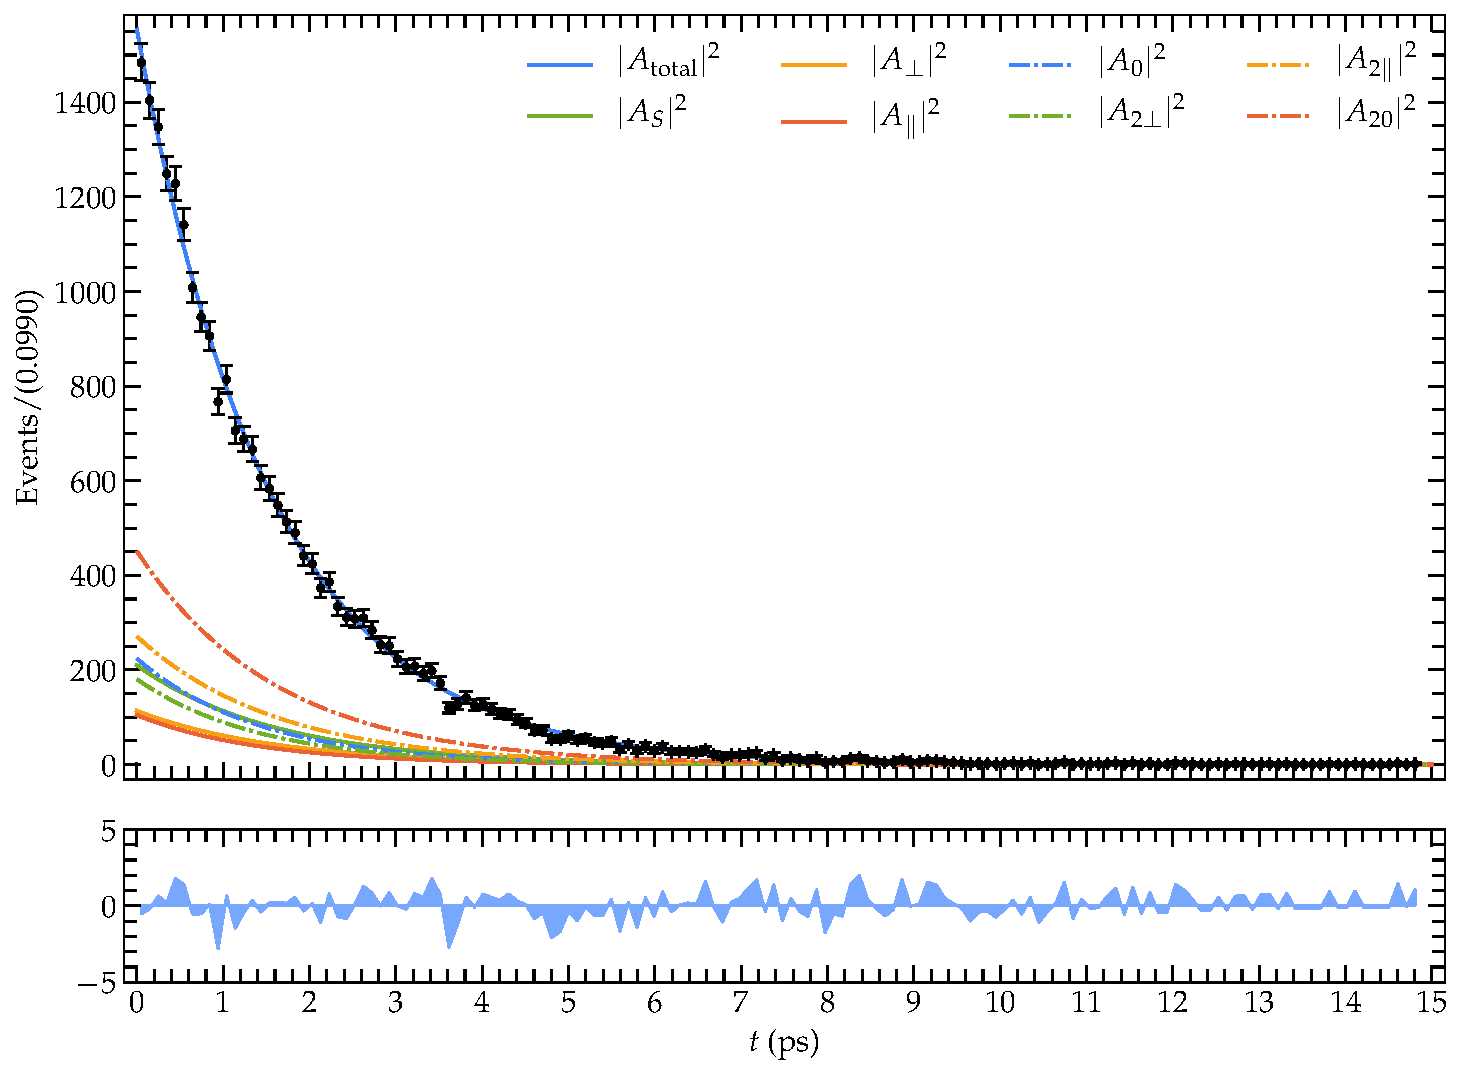
\includegraphics[width=\columnwidth]{plots/20190221c/20190221c_mKK3_Time}
\end{multicols}
\vspace*{-0.5cm}
\caption{Gráficos del ajuste con onda D para el bin $m_{\text{KK}3} = [1.4,1.6)$ GeV.}  
\end{figure}

\begin{figure}[H]
\centering
\begin{multicols}{2}
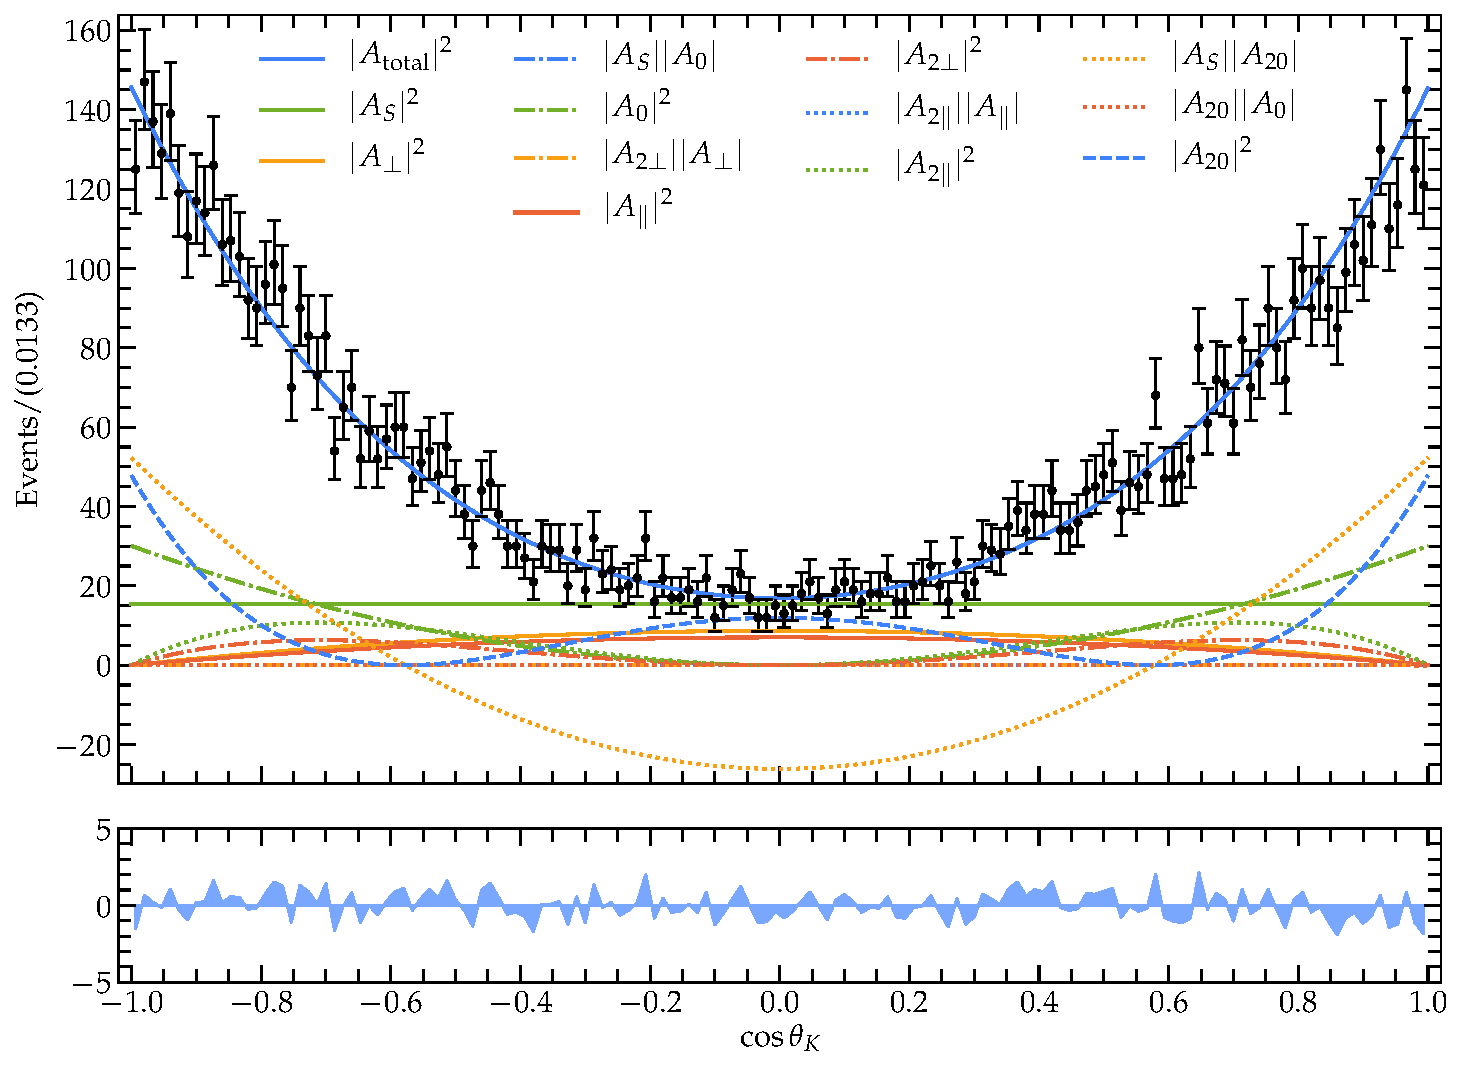
\includegraphics[width=\columnwidth]{plots/20190221c/20190221c_mKK4_CosK}
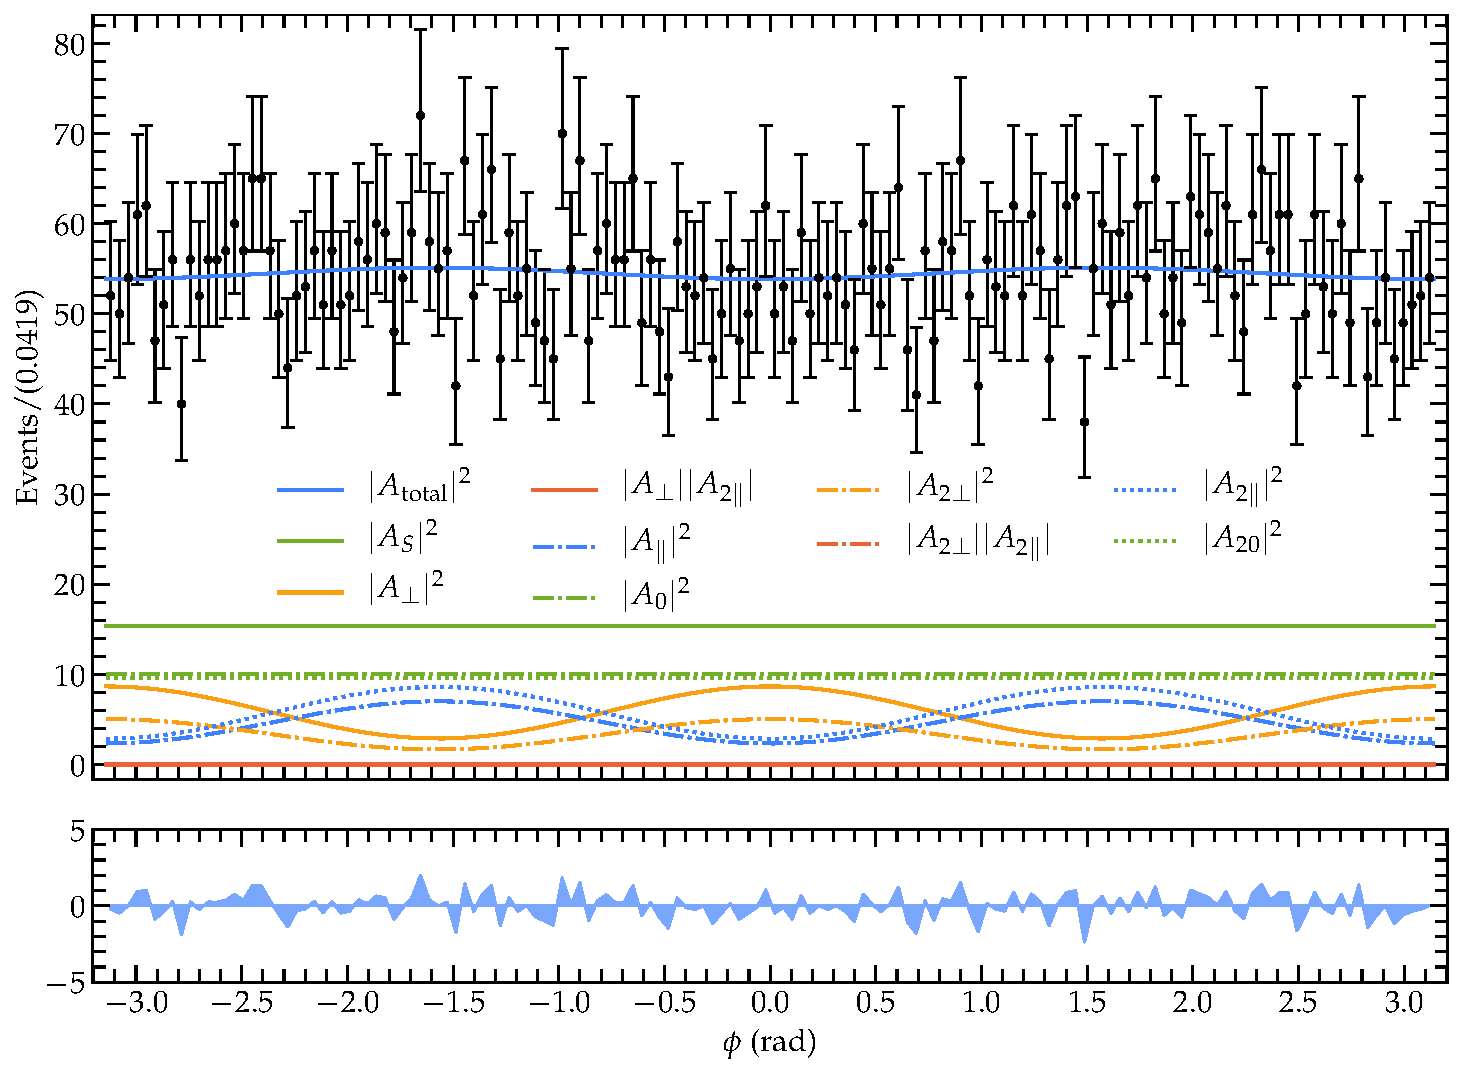
\includegraphics[width=\columnwidth]{plots/20190221c/20190221c_mKK4_Phi}
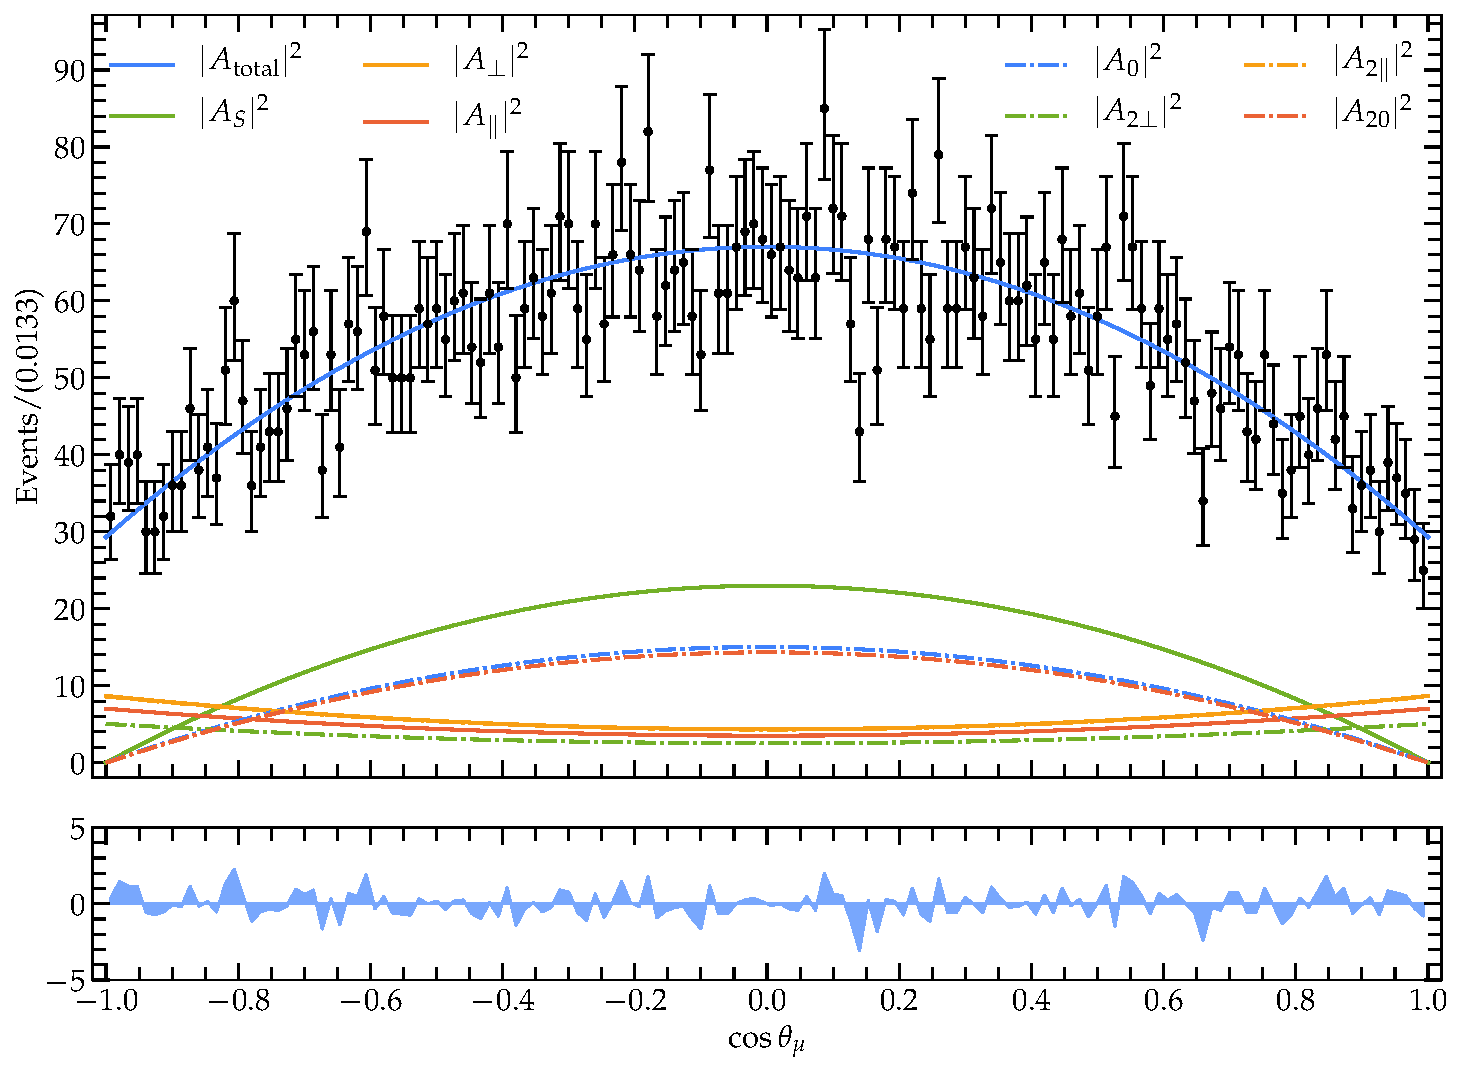
\includegraphics[width=\columnwidth]{plots/20190221c/20190221c_mKK4_CosMu}
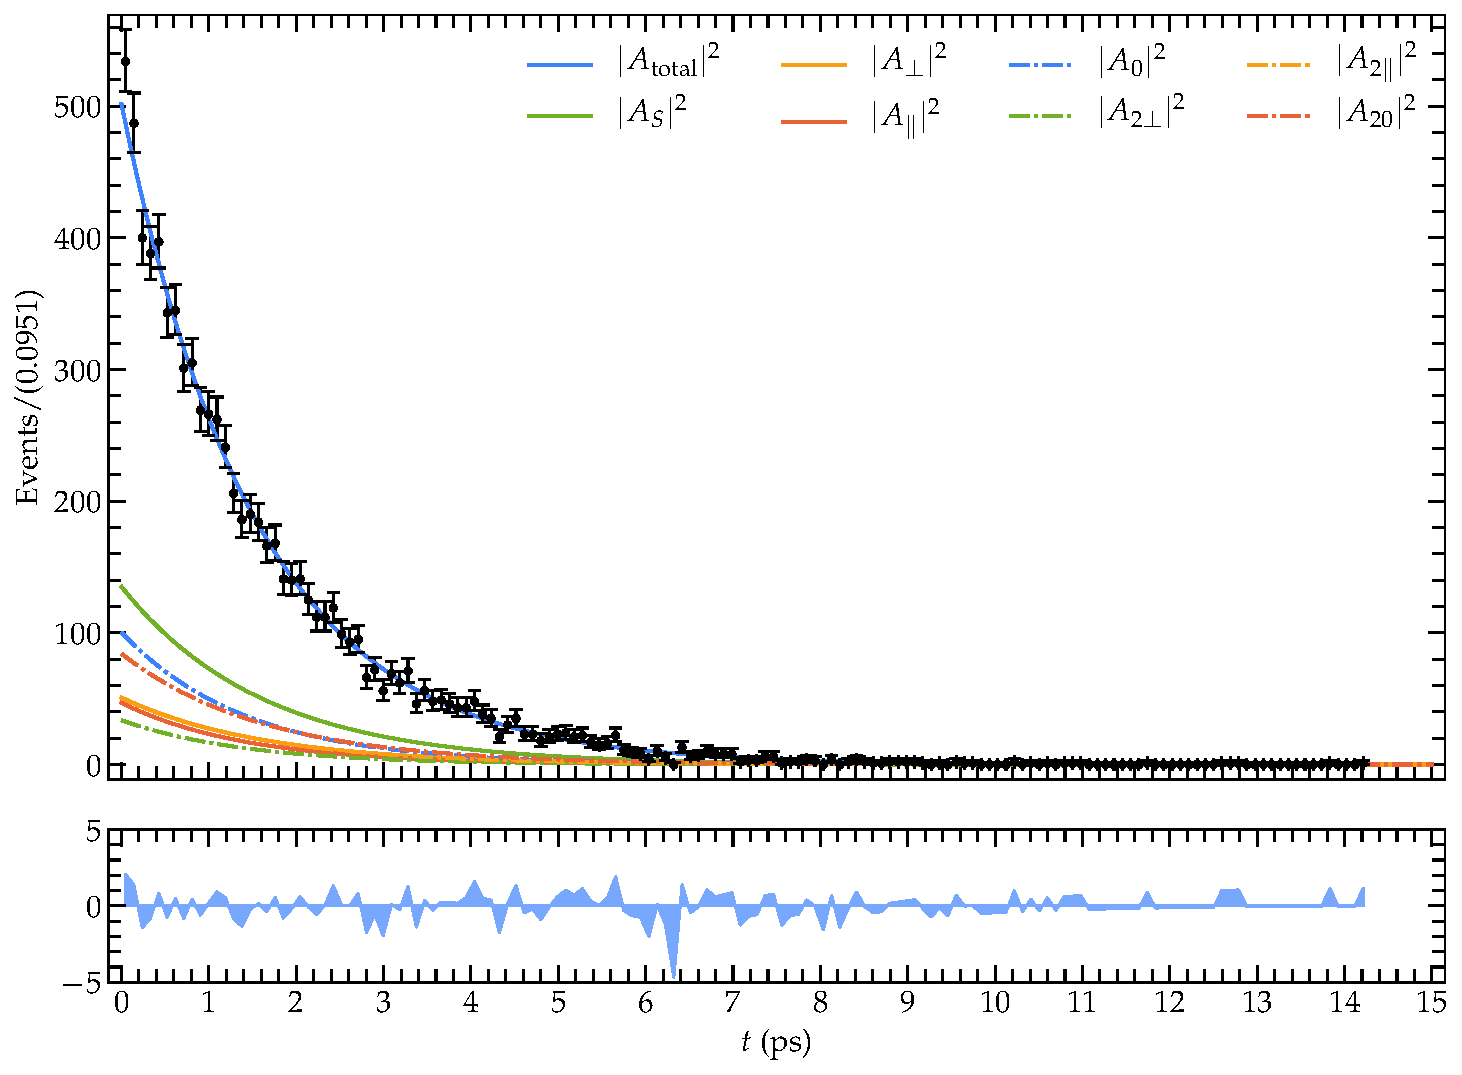
\includegraphics[width=\columnwidth]{plots/20190221c/20190221c_mKK4_Time}
\end{multicols}
\vspace*{-0.5cm}
\caption{Gráficos del ajuste con onda D para el bin $m_{\text{KK}4} = [1.6,1.8)$ GeV.}  
\end{figure}

\begin{figure}[H]
\centering
\begin{multicols}{2}
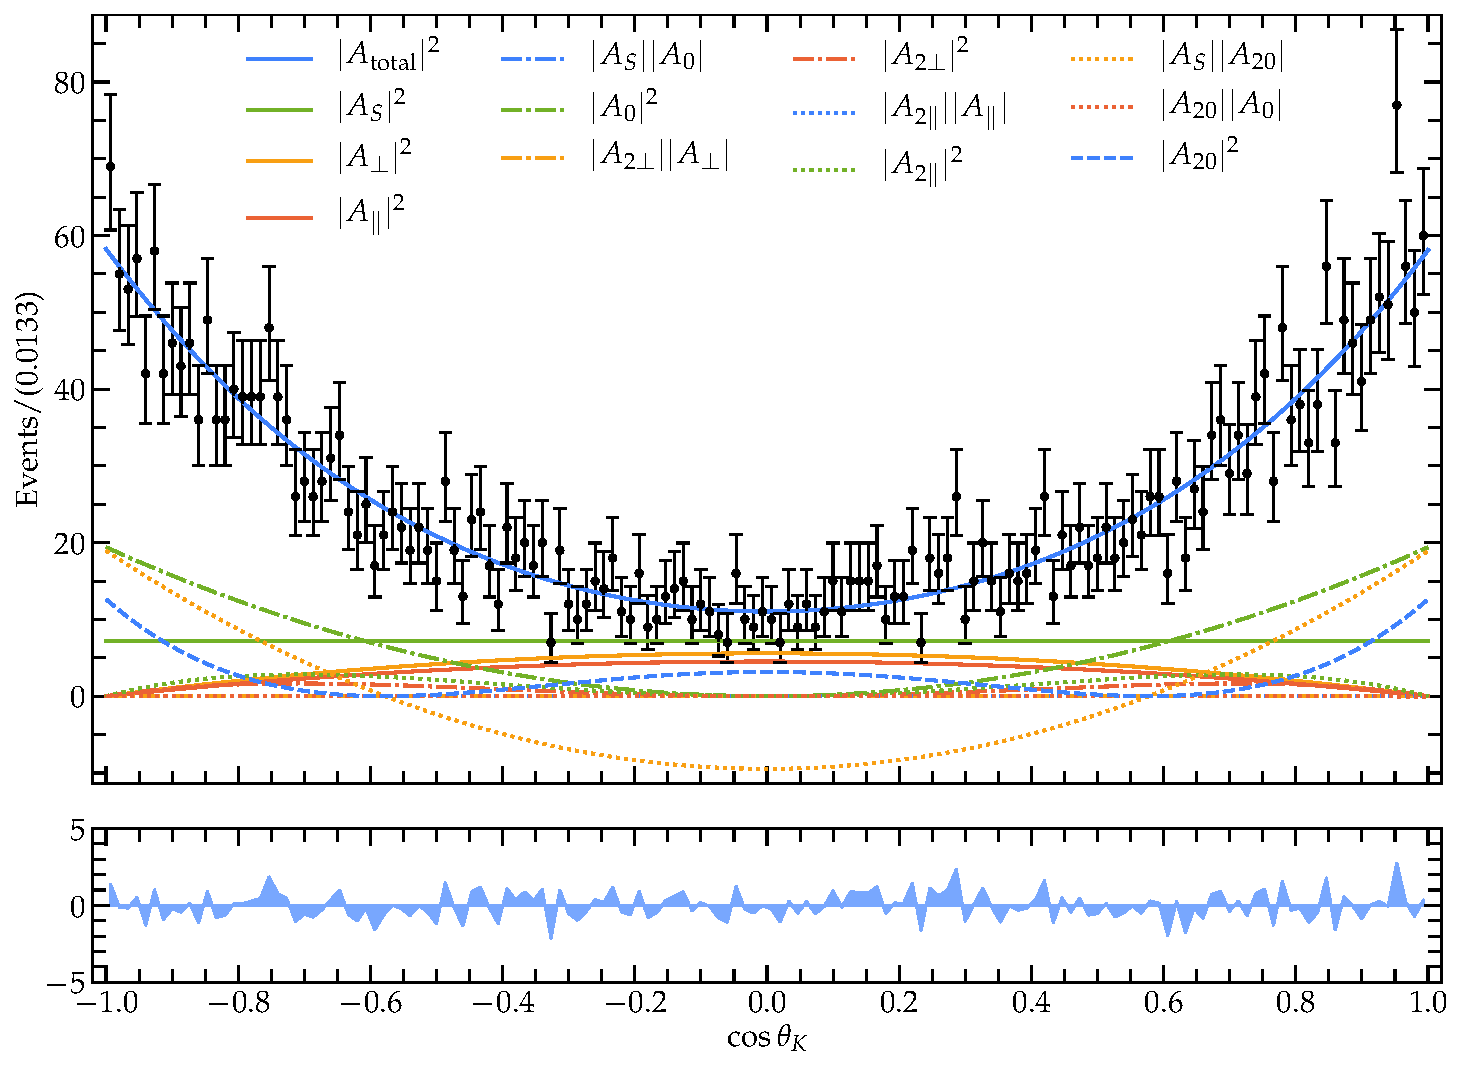
\includegraphics[width=\columnwidth]{plots/20190221c/20190221c_mKK5_CosK}
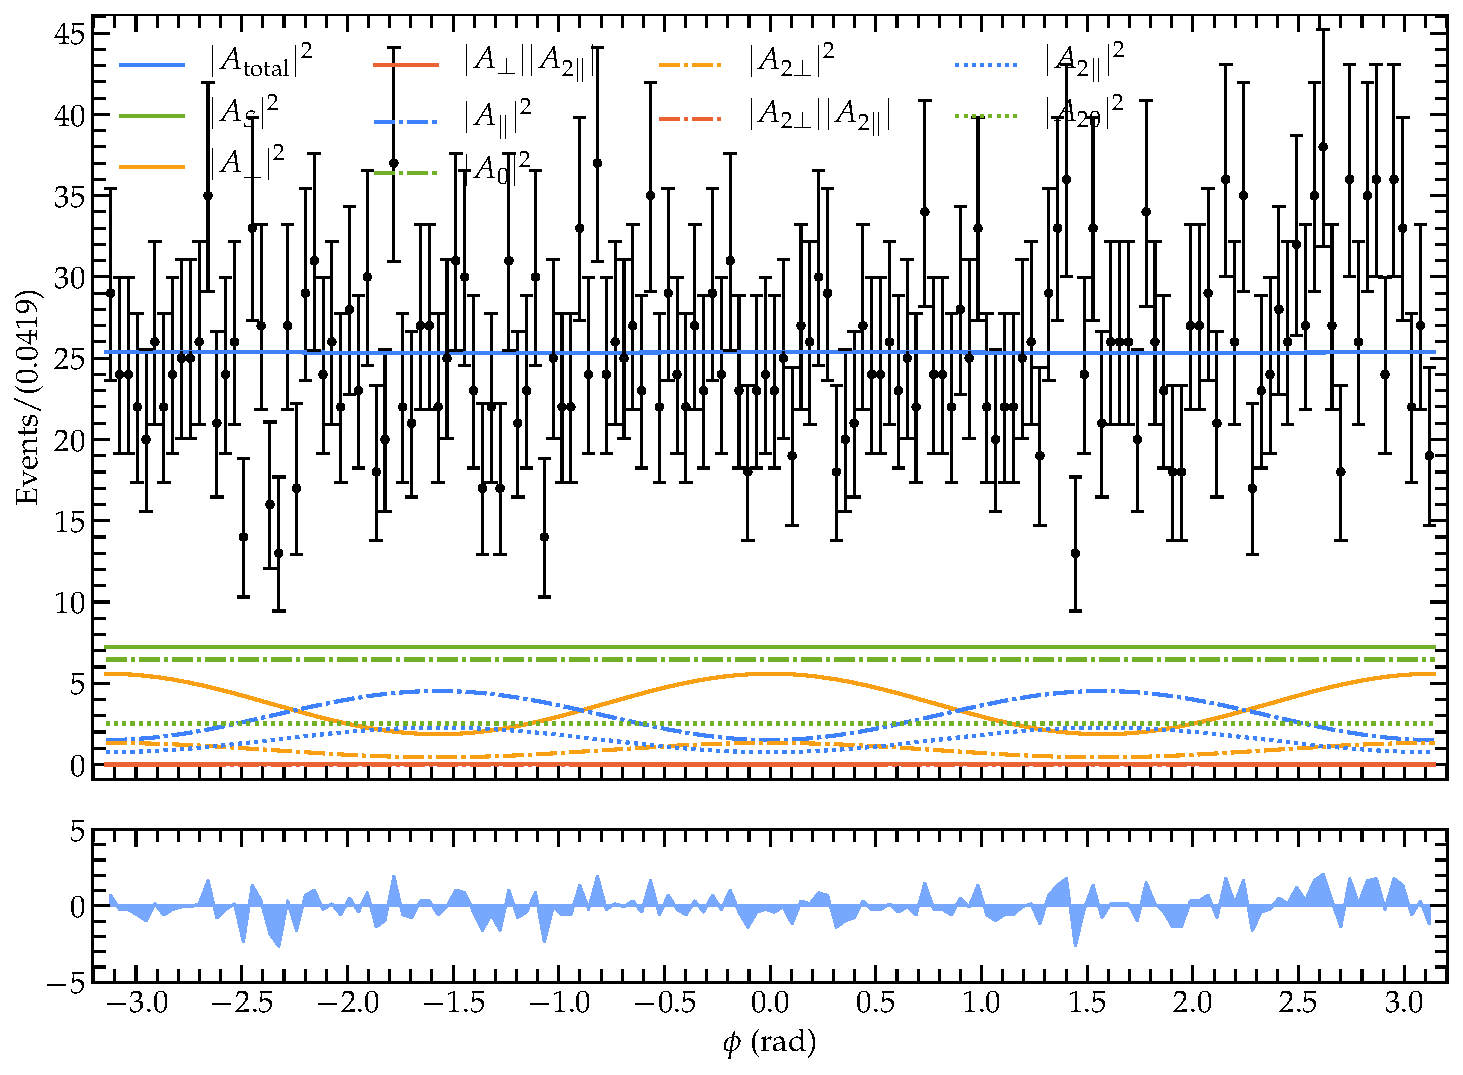
\includegraphics[width=\columnwidth]{plots/20190221c/20190221c_mKK5_Phi}
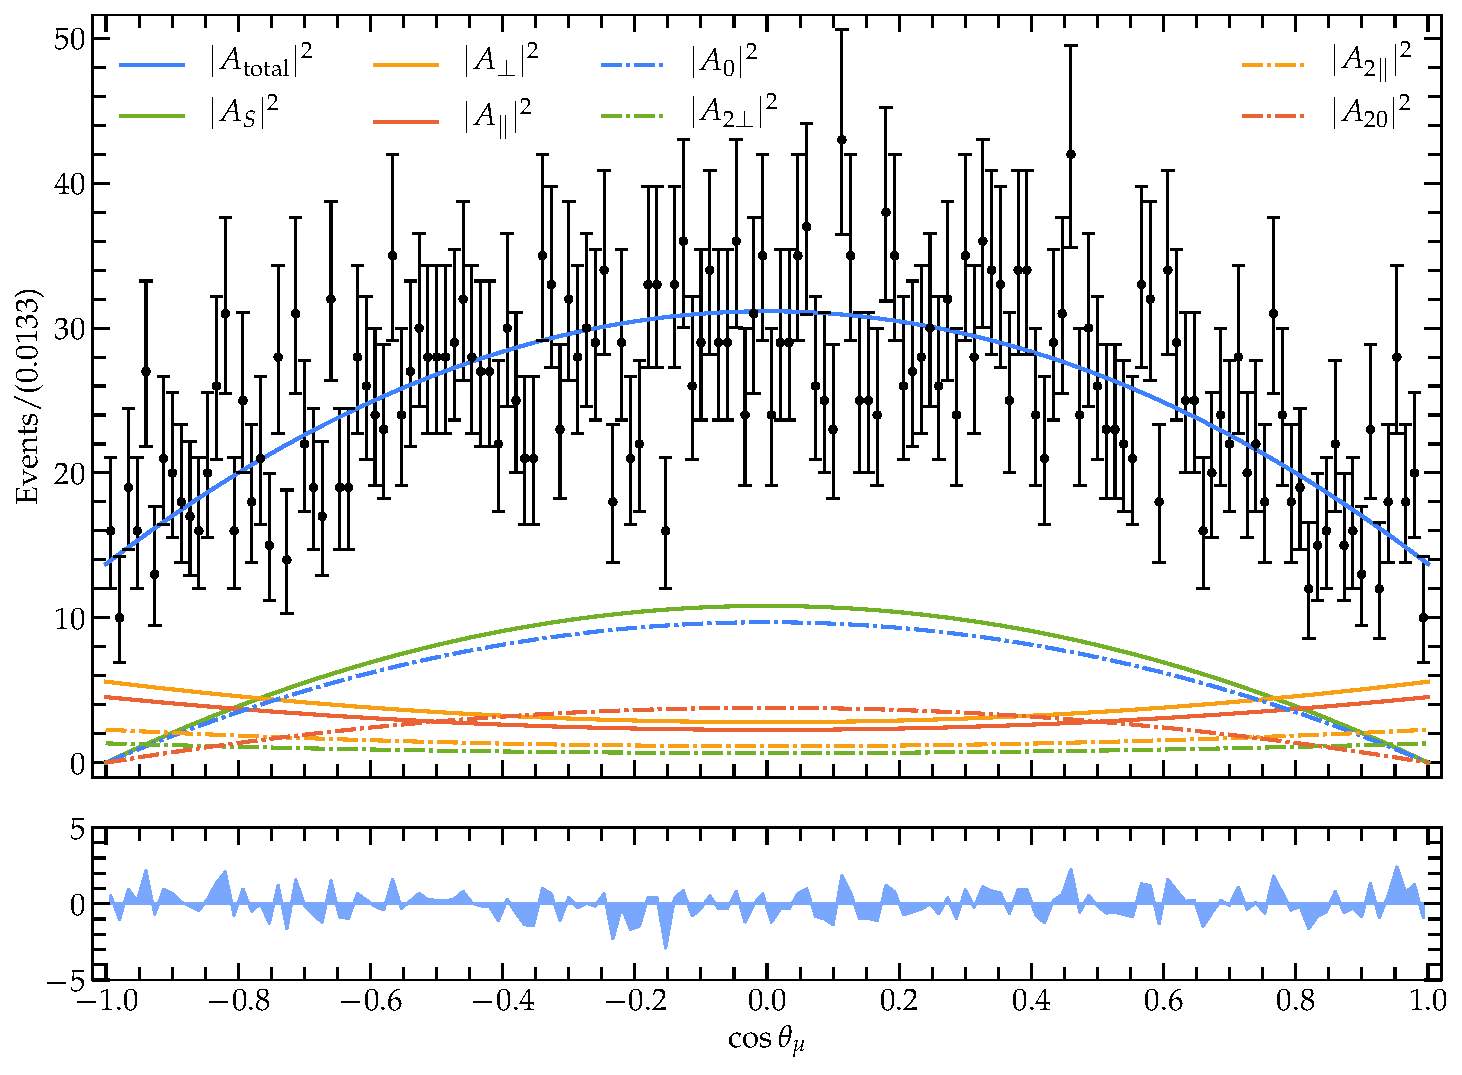
\includegraphics[width=\columnwidth]{plots/20190221c/20190221c_mKK5_CosMu}
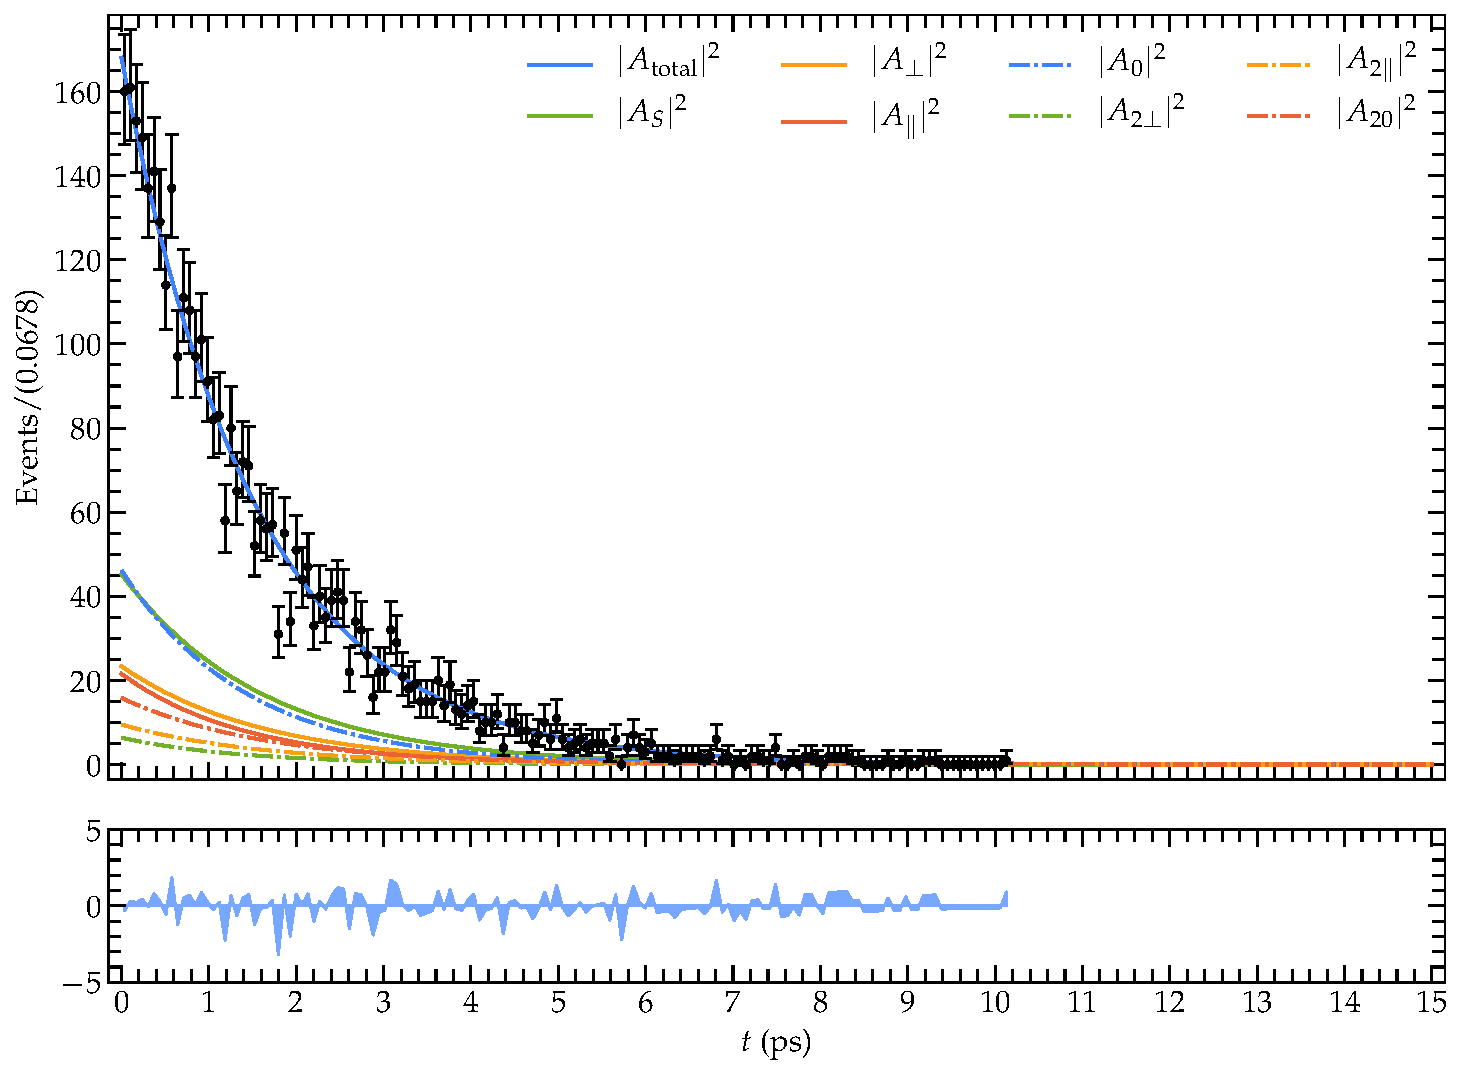
\includegraphics[width=\columnwidth]{plots/20190221c/20190221c_mKK5_Time}
\end{multicols}
\vspace*{-0.5cm}
\caption{Gráficos del ajuste con onda D para el bin $m_{\text{KK}5} = [1.8,2.0)$ GeV.}  
\end{figure}

\begin{figure}[H]
\centering
\begin{multicols}{2}
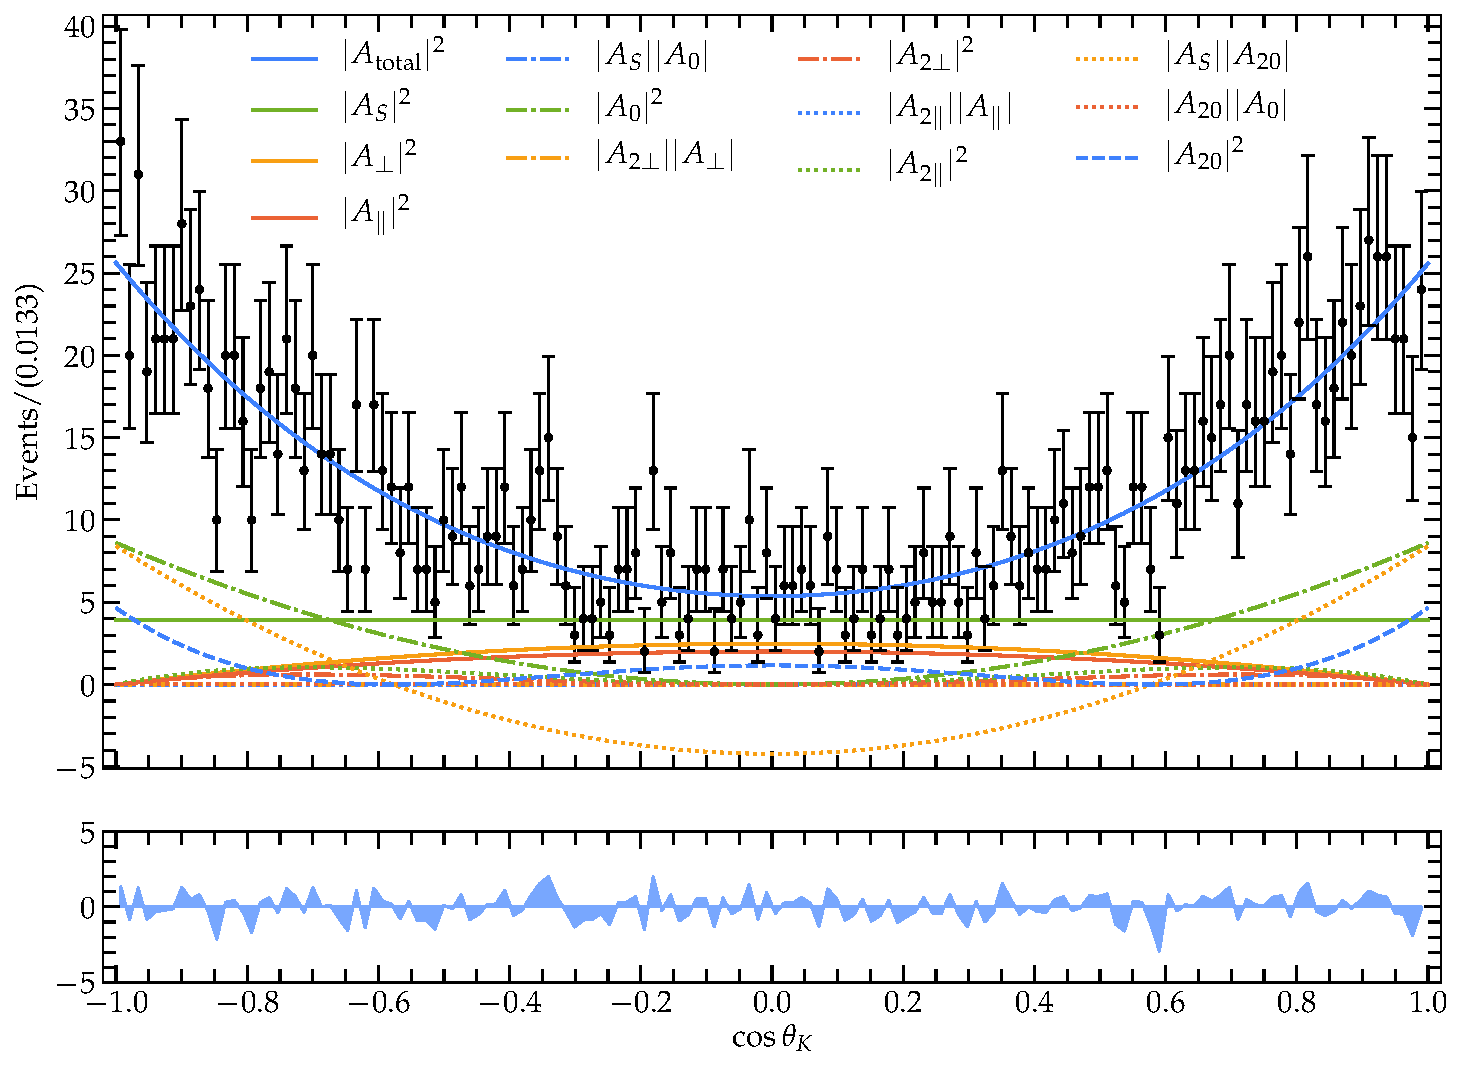
\includegraphics[width=\columnwidth]{plots/20190221c/20190221c_mKK6_CosK}
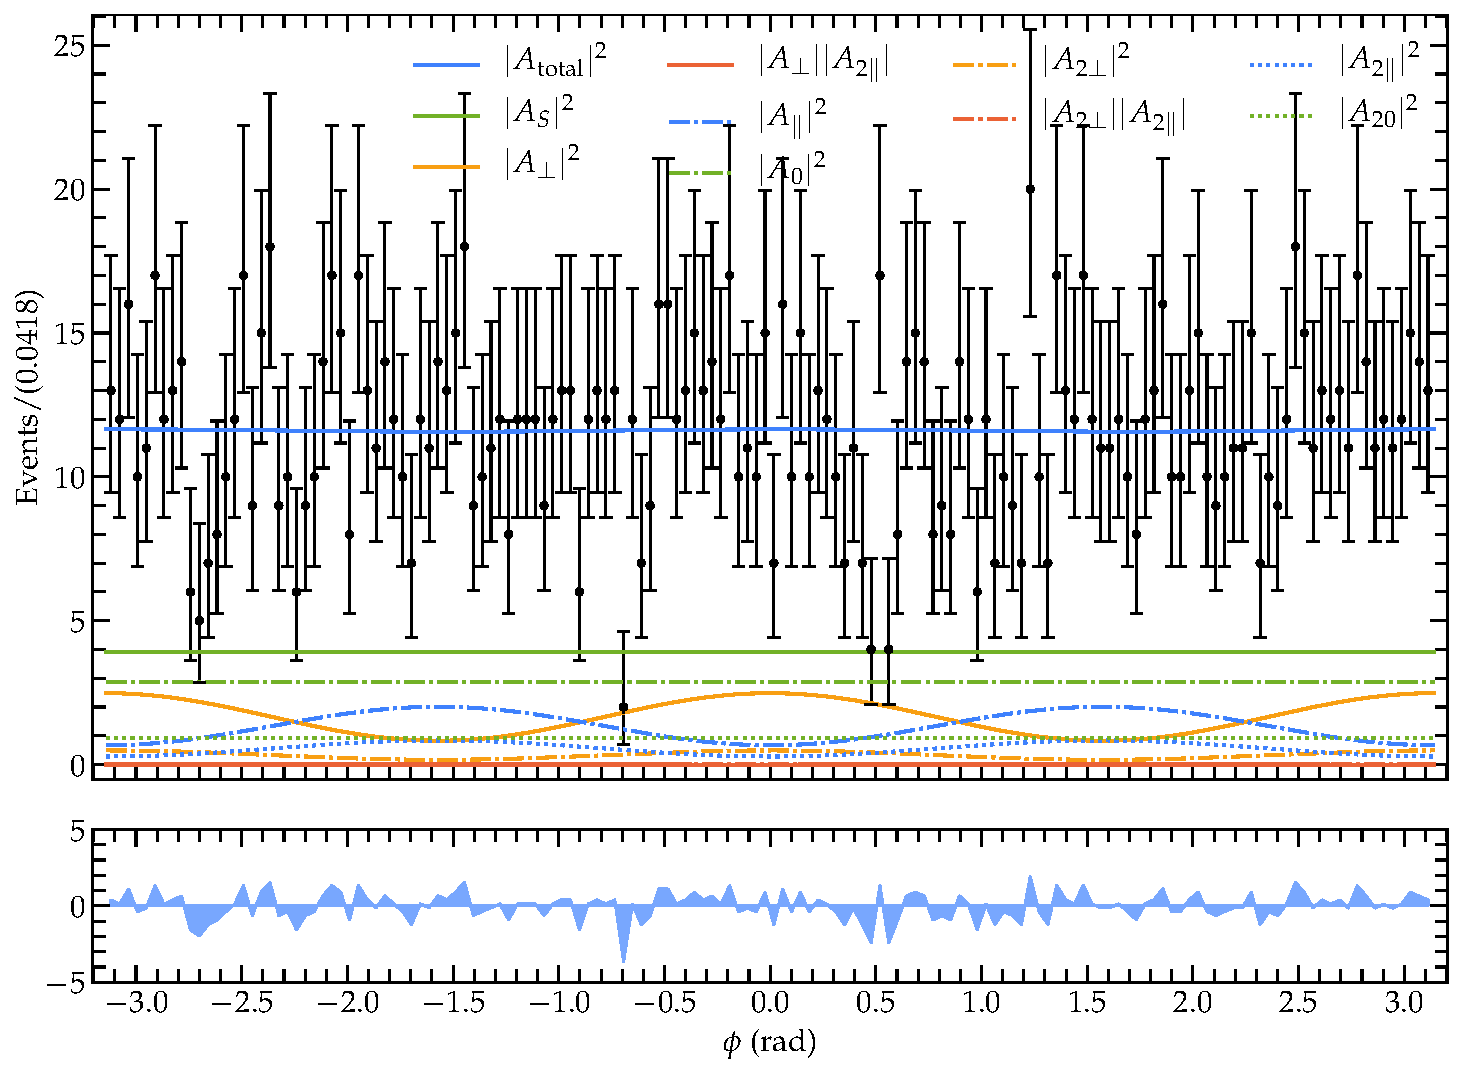
\includegraphics[width=\columnwidth]{plots/20190221c/20190221c_mKK6_Phi}
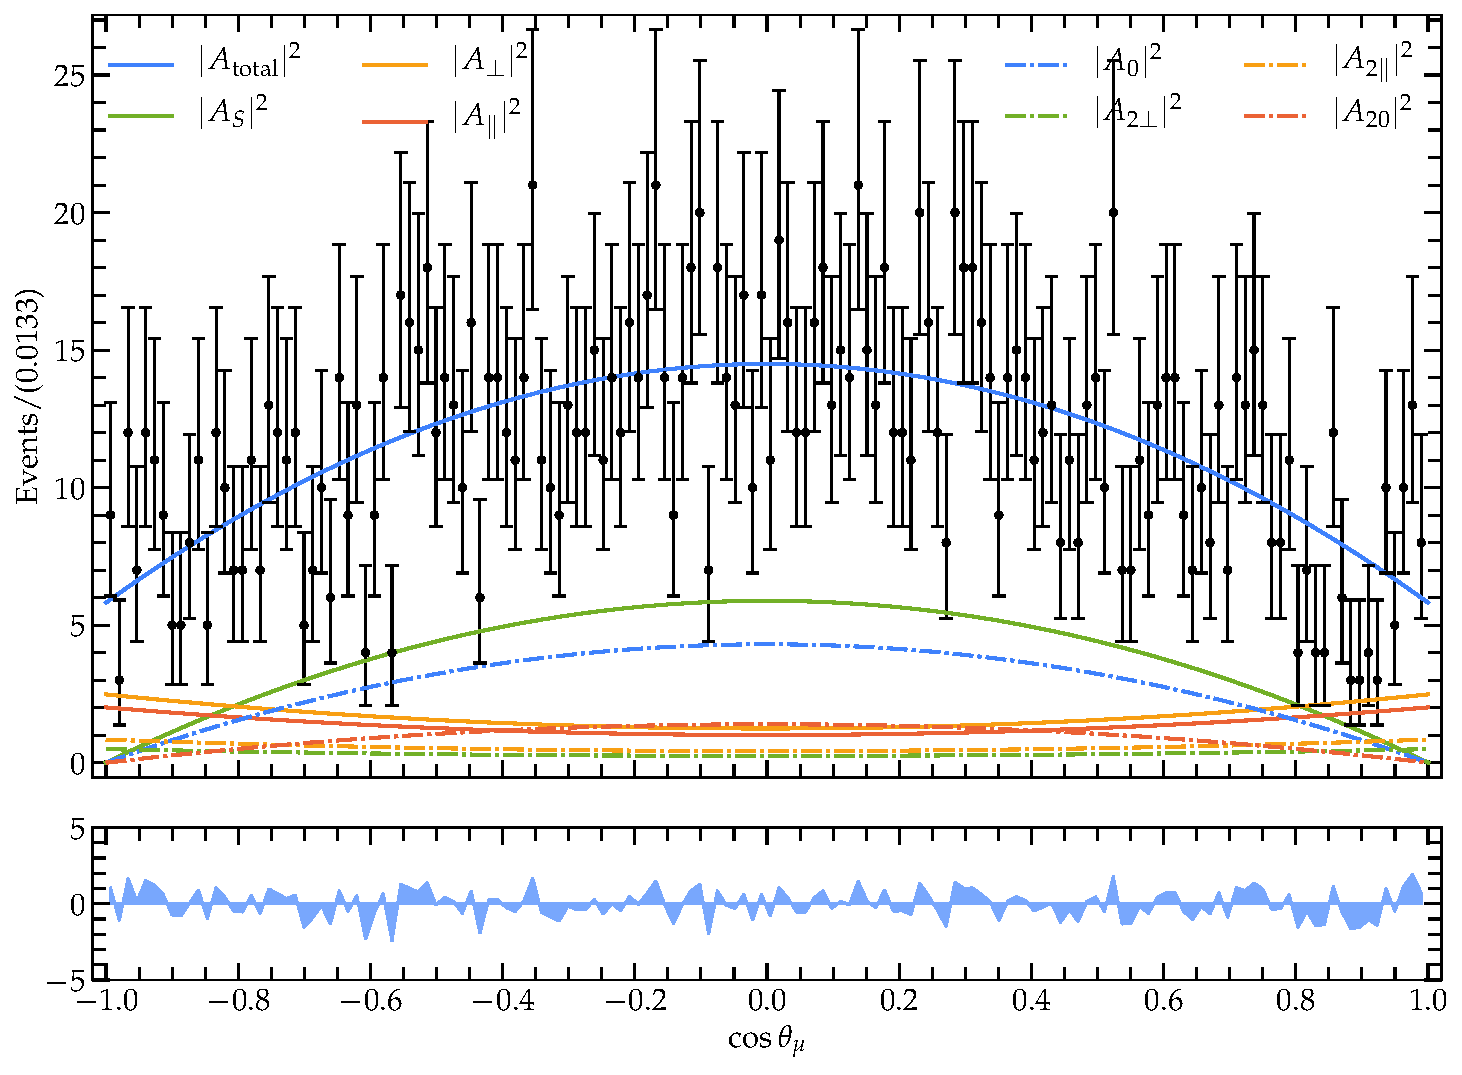
\includegraphics[width=\columnwidth]{plots/20190221c/20190221c_mKK6_CosMu}
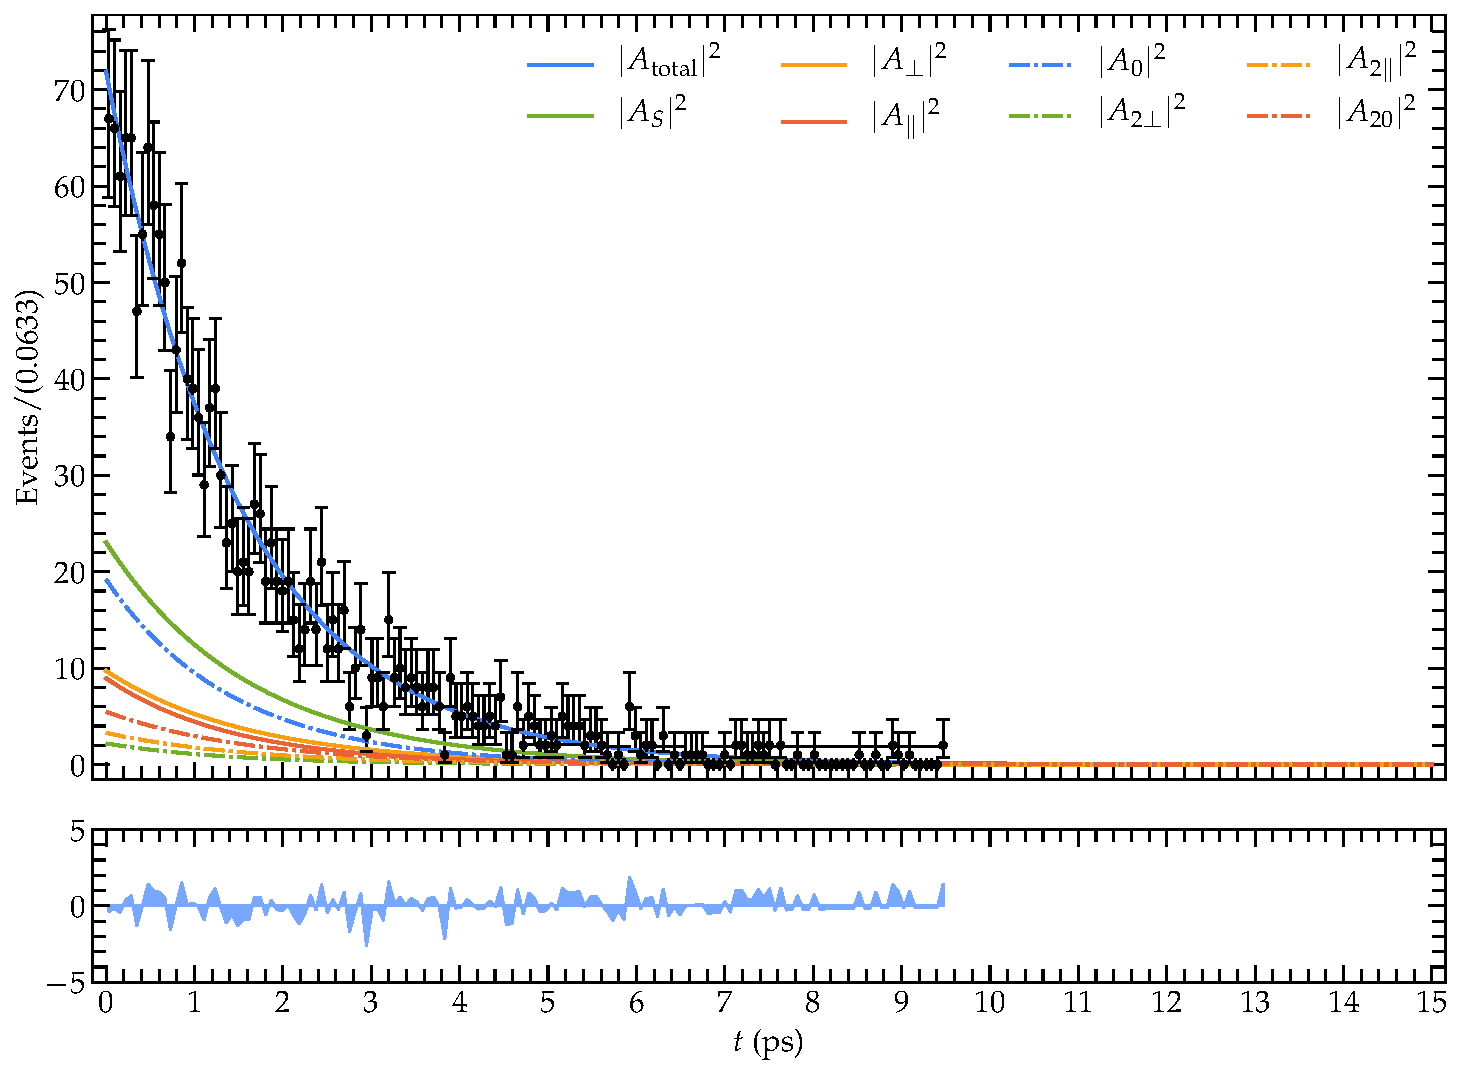
\includegraphics[width=\columnwidth]{plots/20190221c/20190221c_mKK6_Time}
\end{multicols}
\vspace*{-0.5cm}
\caption{Gráficos del ajuste con onda D para el bin $m_{\text{KK}6} = [2.0,2.2)$ GeV.}  \label{fig:20190221c_mKK6}
\end{figure}




